\documentclass[12pt, a4paper, sectionentrydots=true, listof=totoc, listof=entryprefix, numbers=endperiod]{scrartcl}
%
% ============================================================================
% Die Präambel des Dokumentes:
% ============================================================================
%
% In dieser Zeile werden verschiedene Einstellungen zum Dokument vorgenommen.
% Dazu gehören. z.B. Papier-Format, Schriftgrösse, etc.
%
% Hinweis zur Kapitelnummerierung: Soll der Punkt hinter der letzten Zahl der
%                                  letzten Kapitel-Nummer nicht vorhanden sein,
%                                  So kann in der Zeile der Eintrag
%
%                                     numbers=endperiod    geändert werden auf
%                                     numbers=noendperiod
% ============================================================================
%
% Definitionen wie Name des Autors, Matrikel-Nr, Datum der Arbeit, etc.
% Diese werden für die Erstellung der Titelseite benötigt. 
% Da zu diesem Zeitpunkt keine Sprach-Packages geladen sind, müssen die Umlaute
% in der "klassischen LaTeX Weise" gesetzt werden.
%
\def\autor{Peter Kessler}
\def\email{peter.kessler@id.ethz.ch}
\def\mtrnr{1234567}
\def\datum{4. Oktober 2021}
\def\titel{\LaTeX}
\def\artderdoku{Tutorial}
\def\ethz{Eidgen\"ossische~Technische~Hochschule~Z\"urich}
\def\department{Department~for~Computer~Science}
\def\institut{Institute for Computing Platforms}
\def\professur{Data Sciences, Data Systems, and Data Services}
\def\professor{Prof. Ce Zhang}
\def\studienjahrgang{2020}
\def\betreuer{Hans Mustermann}
\def\koexaminator{Bodo Bitbeisser}
%
%
%
% ============================================================================
% Ab dieser Stelle nichts verändern, ausser man weiss was man tut.
% ============================================================================
%
\addtokomafont{pageheadfoot}{\linespread{1}\selectfont}
\usepackage[ngerman]{babel}
\usepackage[utf8]{inputenc}
\usepackage[automark,headsepline,footsepline]{scrlayer-scrpage}
\usepackage{lastpage}
\usepackage{geometry}
\usepackage{graphicx}
\usepackage{chngcntr}
\usepackage[table]{xcolor}
\usepackage{booktabs}
\geometry{includehead,tmargin=15mm,bmargin=30mm,lmargin=30mm,rmargin=20mm}
\usepackage{menukeys}
\renewcaptionname{ngerman}{\contentsname}{Inhaltsverzeichnis}
\renewcaptionname{ngerman}{\listfigurename}{Abbildungsverzeichnis}
\renewcaptionname{ngerman}{\listtablename}{Tabellenverzeichnis}
\renewcaptionname{ngerman}{\figurename}{Abb.}
\renewcaptionname{ngerman}{\tablename}{Tab.}
\renewcommand*\listoflofentryname{\bfseries\figurename}
\BeforeStartingTOC[lof]{\renewcommand*\autodot{:}}
\renewcommand*\listoflotentryname{\bfseries\tablename}
\BeforeStartingTOC[lot]{\renewcommand*\autodot{:}}
\usepackage{setspace}
\clearpairofpagestyles
\pagestyle{scrheadings}
\renewcommand{\sectionmarkformat}{}
\ohead{\rightmark}
\ofoot{Seite \thepage{} von \pageref{LastPage}}
\usepackage{paralist}
\usepackage{enumitem}
\usepackage{courier}
\usepackage{fontenc}
\usepackage{tcolorbox}
\usepackage{ulem}
%
%
%
% ============================================================================
% Package für Symbole:
% ============================================================================
%
\usepackage{amsmath, amssymb}
\usepackage{bm}
%
%
%
% ============================================================================
% An dieser Stelle wird die Darstellung der Links im Dokument eingestellt. 
% ============================================================================
%
%\usepackage[colorlinks=true]{hyperref}
%\usepackage[colorlinks=false]{hyperref}
%\usepackage[hidelinks]{hyperref}
%\usepackage[colorlinks=true, urlcolor=blue, linkcolor=blue, pdfborder={0 0 0}]
%\usepackage[colorlinks=true, urlcolor=blue, allcolors=blue, pdfborder={0 0 0}]{hyperref}
\usepackage[colorlinks=true, urlcolor=blue, allcolors=black, pdfborder={0 0 0}]{hyperref}
\newcommand*{\fullref}[1]{\hyperref[{#1}]{\autoref*{#1} \nameref*{#1}}}
\usepackage[ngerman]{cleveref}
%
%
%
% ============================================================================
% Abkürzungsverzeichnis mit oder ohne Angabe der Seite
% ============================================================================
%
\usepackage[printonlyused]{acronym}
%\usepackage[printonlyused,withpage]{acronym}
%
%
%
% ============================================================================
% Package für Literaturverzeichnis 
% ============================================================================
%
% Für BibLaTex
%\usepackage[numbers]{natbib}
%\bibliographystyle{plainnat}
%\renewcommand*{\bibfont}{\raggedright}
%
%Für Biber in Texmaker
%\usepackage{csquotes}
%\usepackage[backend=biber, style=numeric]{biblatex}
%\addbibresource{./Verzeichnisse/Literatur.bib}
%
%Für Biber in Overleaf
\usepackage{csquotes}
\usepackage{biblatex}
\addbibresource{./Verzeichnisse/Literatur.bib}
%
%
%
% ============================================================================
% Package für Tabellen:
% ============================================================================
%
\usepackage{tabularx}
\newcolumntype{R}[1]{>{\raggedleft\arraybackslash}p{#1}}
\newcolumntype{C}[1]{>{\centering\arraybackslash}p{#1}}
%
%
%
% ============================================================================
% Package für Fussnoten als Endnoten:
% ============================================================================
%
\usepackage{endnotes} 
\renewcommand\enoteformat{\rightskip=0pt \leftskip=0pt \parindent=0em
  \leavevmode\makeenmark\raggedright}
\let\footnote=\endnote
%
%
%
% ============================================================================
% Package für Stichwortverzeichnis:
%
% Für ein Einspaltiges Stichwortverzeichnis: \usepackage[columns=1]{idxlayout}
% Für ein Zweispaltiges Stichwortverzeichnis: \usepackage{idxlayout}
% ============================================================================
%
\usepackage{makeidx}
%\usepackage{idxlayout}
\usepackage[columns=1]{idxlayout}
\makeindex
%
%
%
% ============================================================================
% Variable für die Speicherung der römischen Seitenzahl, 
% damit im Anhang damit weitergefahren werden kann:
% ============================================================================
%
\newcounter{SeitenzahlSpeicherRoman}
%
%
%
% ============================================================================
% Ende Präambel
% ============================================================================
%
\begin{document}
%
% ============================================================================
% Start des Dokumentes 
% ============================================================================
%
% Ab hier sind die einzelnen Kapitel definiert. Das Dokument ist so
% aufgebaut, dass an in dieser Datei lediglich die Reihenfolge der Kapitel
% und die Formate definiert sind. Die eigentlichen Inhalte (sofern diese
% nicht durch LaTeX generiert werden (z.B. Inhaltsverzeichnis, etc.) 
% sind in separaten Dateien enthalten und werden von LaTeX bei der 
% Erstellung des Dokumentes eingelesen.  
%
%
%
% ============================================================================
% Einstellung für die Darstellung der Abschnitte:
% ============================================================================
%
% parindent 
%   - definiert den Einzug (Einrückung) für die erste Zeile von
%     Abschnitten (Pargraphen)
%
% parskip 
%   - definiert den Abstand zwischen den einzelnen Abschnitten 
%
\setlength{\parindent}{0em}
\setlength{\parskip}{0.75em}
%
%
%
% ============================================================================
% Um Texte mit dem Tag \code{} grau hinterlegen zu können
% ============================================================================
%
\definecolor{light-gray}{gray}{0.95}
\newcommand{\code}[1]{\colorbox{light-gray}{\texttt{#1}}}
%
%
%
% ============================================================================
% Erstellen der Titelseite
% ============================================================================
%
\begin{titlepage}
\begin{center}
  \vspace*{3cm}
  \line(1,0){430}\\
  [8mm]
  \huge \textbf{\textsf{\titel}} \\
  [2mm]
  \line(1,0){430}\\
  \vspace{1.5cm}
  \large\textbf{\artderdoku}\\
  \vspace{0.1cm}
  \normalsize
  erstellt am: \datum \\
  \vspace{1.5cm}
  \large \textbf{\department \\ \ethz}\\
  \vfill
\end{center}

\normalsize{
  \begin{tabular}{ll}
    Autor:              & \autor \\
    Matrikelnummer:     & \mtrnr \\
    eMail:              & \email \\
    Institut:           & \institut \\
    Professur:          & \professur \\
    Professor:          & \professor \\
    Studienjahrgang:    & \studienjahrgang \\
    Betreuer:           & \betreuer \\
    Ko-Examinator:      & \koexaminator \\
  \end{tabular}
}

\end{titlepage}
%
%
%
% ============================================================================
% Für die ersten Seiten mit Inhaltsverzeichnis, etc.
% die Seitenzahlen auf römisch einstellen
%
%    \pagenumbering{Roman} = Grossbuchstaben wie I, IV, X
%    \pagenumbering{roman} = Kleinbuchstaben wie i, iv, x
%
% ============================================================================
%
\setcounter{page}{1}
%\pagenumbering{Roman}
\pagenumbering{roman}
\ofoot{\thepage{}}
%
%
%
% ============================================================================
% Abstract / Summary der Arbeit
%
% Um Titel und Eintrag in Kopfzeile, Inhaltsverzeichnis anzupassen:
%
%  - Kopfzeile der Seite: \markright{Eintrag in Kopfzeile}
%  - Inhaltsverzeichnis:  \addcontentsline{toc}{section}{Eintrag in Inhaltsverz}
%  - Kapitelüberschrift:   \section*{Kapitelüberschrift}
%
% Wird die Kapitelüberschrift mit einem * nach dem Keyword section definiert,
% so wird keine Kapitel-Nummer und kein Eintrag in das Inhaltsverzeichnis
% erstellt. 
% ============================================================================
%
\pagebreak 
\clearpage
\markright{Abstract / Summary}
\clearpage
\section*{Abstract / Summary}
\addcontentsline{toc}{section}{Abstract / Summary}
\begin{spacing}{1.25} 
Dieses Dokument (erstellt mit \LaTeX\ - siehe Kapitel:  \nameref{Installation} auf Seite \pageref{Installation}), soll die Erstellung von umfangreichen technischen oder wissenschaftlichen Dokumentationen erleichtern.

\begin{tcolorbox}
Are you ready to leave those \dq what you see is what you get\dq{} word processors behind and to enter the world of real, reliable, and high-quality typesetting\cite{Kottwitz2011}?
\end{tcolorbox}

Ob in Uni, Beruf oder Alltag: Muss eine umfangreiche technische oder wissenschaftlich Dokumentation erstellt werden, führt über kurz oder lang kein Weg an \LaTeX\ vorbei.\par  

\textbf{Wofür eignet sich \LaTeX?}
\begin{compactitem}
\item jede Art wissenschaftlicher Veröffentlichungen 
\item Bücher (Sachbücher, Romane, Lexika, ...) 
\item Lebensläufe, Serienbriefe, Vorträge und Poster 
\item  ... 
\end{compactitem}
\par 

\textbf{Wofür eignet sich \LaTeX\ nicht!}
\begin{compactitem} 
\item Zeitungssatz  
\item Desktop Publishing (Plakate, Flyer etc.)  
\item sehr kurze Texte  
\item alle Bereiche, in denen Seiten-Elemente völlig frei angeordnet werden sollen
\item  ... 
\end{compactitem}
\par 

\LaTeX\ verführt immer wieder viele Anwender – insbesondere Anfänger – dazu, irgendetwas noch schöner zu machen: 'fancy' Schriften zu verwenden, am Layout herumzubasteln, Bilder punktgenau auf einer Seite zu platzieren, etc. Tatsächlich sind die Möglichkeiten nahezu unbegrenzt. Aber: Layout und Schriften sollen nicht schön sein, sondern den Inhalt der Arbeit aus Sicht des Lesers optimal transportieren.\par

\LaTeX\ ist somit nicht geeignet für jemanden, der sagt: 'Ich weiss selber am besten, wie mein Dokument aussehen soll.'. Man kann zwar mit \LaTeX\  im Prinzip alles machen, aber man muss entweder Glück haben und jemand anders hat schon ein entsprechendes Paket geschrieben, das man verwenden kann, oder man muss sehr viel Wissen über \TeX\ haben.\par

\LaTeX\ ist dagegen sehr gut geeignet für alle die sagen 'Ich möchte mich nur um den Inhalt, aber nicht um die Formatierung kümmern. Es soll aber trotzdem gut aussehen.'.\par 

\end{spacing} 
%
%
%
% ============================================================================
% Widmung / Danksagung der Arbeit
% ============================================================================
%
\pagebreak 
\clearpage
\markright{Widmung / Danksagung}
\clearpage
\section*{Widmung / Danksagung} 
\addcontentsline{toc}{section}{Widmung / Danksagung}
\begin{spacing}{1.25}
Der Text für die Widmung resp. die Danksagung kann an dieser Stelle eingefügt werden.

\end{spacing} 
%
%
%
% ============================================================================
% Inhaltsverzeichis der Arbeit
% ============================================================================
%
\pagebreak 
\setuptoc{toc}{totoc}
\begin{spacing}{1.0}
\tableofcontents
\end{spacing}
%
%
%
% ============================================================================
% Abbildungsverzeichnis der Arbeit
% ============================================================================
%
\pagebreak 
\begin{spacing}{1.0}
\listoffigures
\end{spacing}
%
%
%
% ============================================================================
% Tabellenverzeichnis der Arbeit
% ============================================================================
%
\pagebreak 
\begin{spacing}{1.0}
\listoftables
\end{spacing}
%
%
%
% ============================================================================
% Ankürzungen und Abkürzungsverzeichnis
%
%  - Alle Abkürzungen in einem separaten File gem. Vorlage erfassen.
% ============================================================================
% 
\pagebreak 
\clearpage
\markright{Abkürzungsverzeichnis}
\clearpage
\section*{Abkürzungsverzeichnis} 
\addcontentsline{toc}{section}{Abkürzungsverzeichnis}
\begin{acronym}[SEPSEPSEP]
\setlength{\parskip}{0ex}
\acro{eth}[ETH]{Eidgenössische Technische Hochschule}
\acro{ethz}[ETHZ]{Eidgenössische Technische Hochschule Zürich}
\acro{epfl}[EPFL]{École polytechnique fédérale de Lausanne}
\acro{id}[ID]{Informatikdienste}
\acro{pm}[PM]{Portfolio Management}
\acro{ppf}[PPF]{Procurement and Portfolio Management}
\end{acronym}
\pagebreak 
%
%
%
% ============================================================================
% Symbole und Symbolverzeichnis
%
%  - Alle Symbole in einem separaten File gem. Vorlage erfassen.
% ============================================================================
% 
\clearpage
\markright{Symbolverzeichnis}
\clearpage
\section*{Symbolverzeichnis}
\addcontentsline{toc}{section}{Symbolverzeichnis}
\begin{spacing}{1.0}
\begin{table}[h!]
\noindent\begin{tabular}{@{}p{2.5cm}l}
$\mathbf{N}$        & Menge aller natürlichen Zahlen ohne die Null \\
$\mathbf{N}_{0}$    & Menge aller natürlichen Zahlen mit der Null \\
\bm{$\pi$}          & Die Kreiszahl Pi \\
\bm{$\Omega$}       & Der elektrische Widerstand Ohm \\
$\boldsymbol\alpha$ & Alpha, der erste Buchstabe des griechischen Alphabetes \\
\end{tabular}
\end{table}

\end{spacing}
%
%
%
% ============================================================================
% Zwischenspeichern der römischen Seitenzahl, sowie 
% umstellen der Seitenzahlen auf arabisch und starten bei 1
% ============================================================================
%
\setcounter{SeitenzahlSpeicherRoman}{\value{page}}
\clearpage
\setcounter{page}{1}
\pagenumbering{arabic}
\ofoot{- \thepage{} -}
%
%
%
% ============================================================================
% ============================================================================
% ============================================================================
% Hier beginnt der eigentliche (fachliche) Inhalt des Dokumentes
% ============================================================================
% ============================================================================
% ============================================================================
%
% Ab dieser Stelle werden Kapitel und Unterkapitel nummeriert und automatisch
% in das Inhaltsverzeichnis eingetragen (kein * nach dem Keyword section).
%
% Alle Kapitel-Nummern werden mit einem Punkt abgeschlossen:
%    1.  
%    1.1.   
% sollen Die Kapitel ohne Punkt abgeschlossen werden:
%    1
%    1.1
% so kann dies in der Zeile \documentclass eingestellt werden (siehe oben).
%
% Der gesamte Inhaltliche Teil des Dokumentes wird mit Zeilenabstand 1.5
% erstellt. Wo dies nicht erwünscht ist (z.B. Tabellen), wird dies jeweils
% für die Bereiche zurückgestellt auf Zeilenabstand 1. 
%
% Die eigentlichen Inhalte können in separaten Dateien erfasst werden und 
% mit \input{datei_mit_inhalt} eingebunden werden. Beachte dazu auch die
% Struktur des Verzeichnisses das die Arbeit enthällt.
%
% Jedes Kapitel (section) startet auf einer neuen Seite \pagebreak
% Unterkapitel (subsection) starten gem. Inhalt
% ============================================================================
%
%
%
%
%
% ===== Kapitel 1 ======
%
\pagebreak
\section{Installation und Konfiguration der LaTeX-Umgebung} 
%
%
\subsection{Installation der LaTeX-Umgebung} \label{Installation}
\begin{spacing}{1.25}
LaTeX (sprich: Latech) ist ein mächtiges Werkzeug zum Setzen von Schriftstücken. Gerade dann, wenn die Texte etwas länger werden, spielt es seinen entscheidenden Vorteil aus: Anders als andere Textverarbeitungssysteme stürzt es nie ab, auch bei mehr als 1000-seitigen Büchern nicht. Einer der weiteren grossen Vorteile von LaTeX ist es, dass es sich nach der Logik des Dokumentes richtet. LaTeX sagt man nicht \dq dieser Text hier soll etwas grösser und fett sein\dq{} sondern \dq dies hier ist eine Überschrift\dq. Alles andere erledigt LaTeX von selbst. LaTeX verarbeitet den Text teilweise vollautomatisch und nach einigen wenigen Anfangskonfigurationen kann man sich voll und ganz auf den Inhalt konzentrieren, statt sich mit der Formatierungen herumzuschlagen. Hinzu kommt, dass in LaTeX ein sehr leistungsfähiger, einfach zu bedienender Formeleditor eingebaut ist, was LaTeX vor allen Dingen für wissenschaftliche Arbeiten interessant macht. LaTeX wurde ausserdem mit dem Ziel geschrieben, dass Schriftstücke auch in 100 Jahren noch gleich aussehen und nicht so wie bei Textverarbeitungssytemen mal die Zeile auf die nächste Seite rutscht, mal die Bilder verrutschen oder gar nicht mehr da sind. LaTeX-Dokumente zu \dq programmieren\dq{} ist vergleichbar mit Internetseiten mit der Seitenbeschreibungssprache HTML zu programmieren. Es ist ähnlich einfach wie HTML und auch ähnlich aufgebaut. Jedoch ist es nicht für Internetseiten programmiert, sondern für beliebige Papierdokumente. Last but not least ist ein ausschlaggebendes Argument für LaTeX, dass es völlig kostenlos ist. 

Leider bringt LaTeX auch einen grossen Nachteil mit sich, den ich hier nicht verschweigen will. LaTeX muss man sozusagen \dq programmieren\dq. 

\begin{figure}[h!]
\centering
  
\includegraphics[width=0.5\textwidth]{./Bilder/LaTeX_Anwender.jpg}
  \caption{Arbeiten mit \LaTeX}
\end{figure}

Einige Befehle sind zu erlernen. Wenn man einen gewissen Befehlssatz auswendig kann, dann gewinnt dieses \dq Programmieren\dq{} jedoch einen riesigen Geschwindigkeitszuwachs, so dass \dq normale \dq{} Text\-ver\-ar\-beit\-ungs\-systeme nicht mehr mithalten können. LaTeX ist auch nicht für hochgradige Designer-Texte geeignet. Der Designer kümmert sich um das Aussehen der Seite. Gerade dies ist bei LaTeX dem LaTeX-Übersetzer überlassen. 

LaTeX-Dokumente werden im Allgemeinen mittels einer Entwicklungsumgebung erstellt. Zwar kann man LaTeX-Dokumente auch mit Hilfe eines einfachen Texteditors erfassen und auf der Kommandozeile das Dokument erstellen. Doch bieten die auf LaTeX angepassten Programme mehr Funktionen und Komfort. Viele LaTeX-Befehle, Sonderzeichen und Symbole sind über die grafische Benutzeroberfläche zugänglich, und teilweise lassen sich darüber auch einfache Tabellen erstellen. Für grosse Projekte bieten Entwicklungsumgebungen eine Verwaltung und Strukturdarstellung. Dokumentenvorlagen und PDF-Vorschau finden sich fast überall. Zur Verbesserung der Lesbarkeit des Codes gibt es eine Syntax-Hervorhebung und teilweise auch eine Autovervollständigung von Befehlen. Manche Programme bieten eine Rechtschreibprüfung. Umlaute werden von manchen Entwicklungsumgebungen automatisch in LaTeX-Befehle übersetzt. Der fortschrittlichere Ansatz zur Verwendung von Umlauten ist eine geeignete Zeichenkodierung und ein dazu passendes LaTeX-Paket. Manche Umgebungen unterstützen insbesondere Unicode. 

Da LaTeX ein freies Produkt ist, welches auch im Sourcecode verfügbar ist, gibt es viele unterschiedliche sogenannte Distributionen. Das System wurde ehemals für den Unixbereich entwickelt, wurde aber auf sehr viele Systeme übertragen.

\textbf{MikTex\index{MikTex}} ist eine sehr gute LaTeX-Distribution für Windows. Während der Installation wird nachgefragt, wie mit fehelnden Packages umgegangen wird. Es ist empfohlen, diese mit Nachfrage installieren zu lassen, da bei der erstmaligen Übersetzung dieses Dokumentes werden so einige Packages nach-installiert. Diese sind jedoch für ein korrektes Layout und für die korrekte Funktionsweise notwendig. Der Installer dieser Distribution ist erhältlich unter  \code{\url{https://miktex.org/}}

\textbf{Texmaker\index{Texmaker}} ist ein plattformübergreifender Unicode-Texteditor für die Erstellung von LaTeX-Dokumenten. Die Software wird unter der GNU General Public License ver\-öf\-fent\-licht. Texmaker ist sehr gut bedienbar und übersichtlich. Ähnlich zu den anderen bekannten LaTeX - Editoren bietet auch er die grundlegende Unterstützung beim Einfügen von LaTeX-Konstruktionselementen - jedoch noch einige weitere Besonderheiten. Der Editor richtet sich insbesondere an LaTeX-Anfänger, denen mit Hilfe von Assistenten die Erstellung von Dokumenten erleichtert werden soll. Details und weiteres findet man unter \code{\url{http://www.xm1math.net/texmaker/}}

Dieses Tutorial/Template ist mit \textbf{Overleaf} erstellt worden. 

\end{spacing}
%
%
\subsection{Konfiguration der LaTeX-Umgebung} \label{Konfiguration}
\begin{spacing}{1.25}
LaTeX nimmt die *.tex Datei(en) und erstellt damit die eigentliche Druck-Datei (z.B. *.pdf). Dieser Vorgang ist nicht trivial. Abhängig von den gewünschten Ergebnissen resp. der zu erstellenden Verzeichnisse, muss der Übersetzungsvorgang mehrfach ausgeführt werden damit letztendlich das Dokument wie gewünscht erstellt wird.

Texmaker ist via \menu{Optionen > Texmaker konfigurieren} wie folgt zu konfigurieren:

\begin{figure}[h!]
\centering
  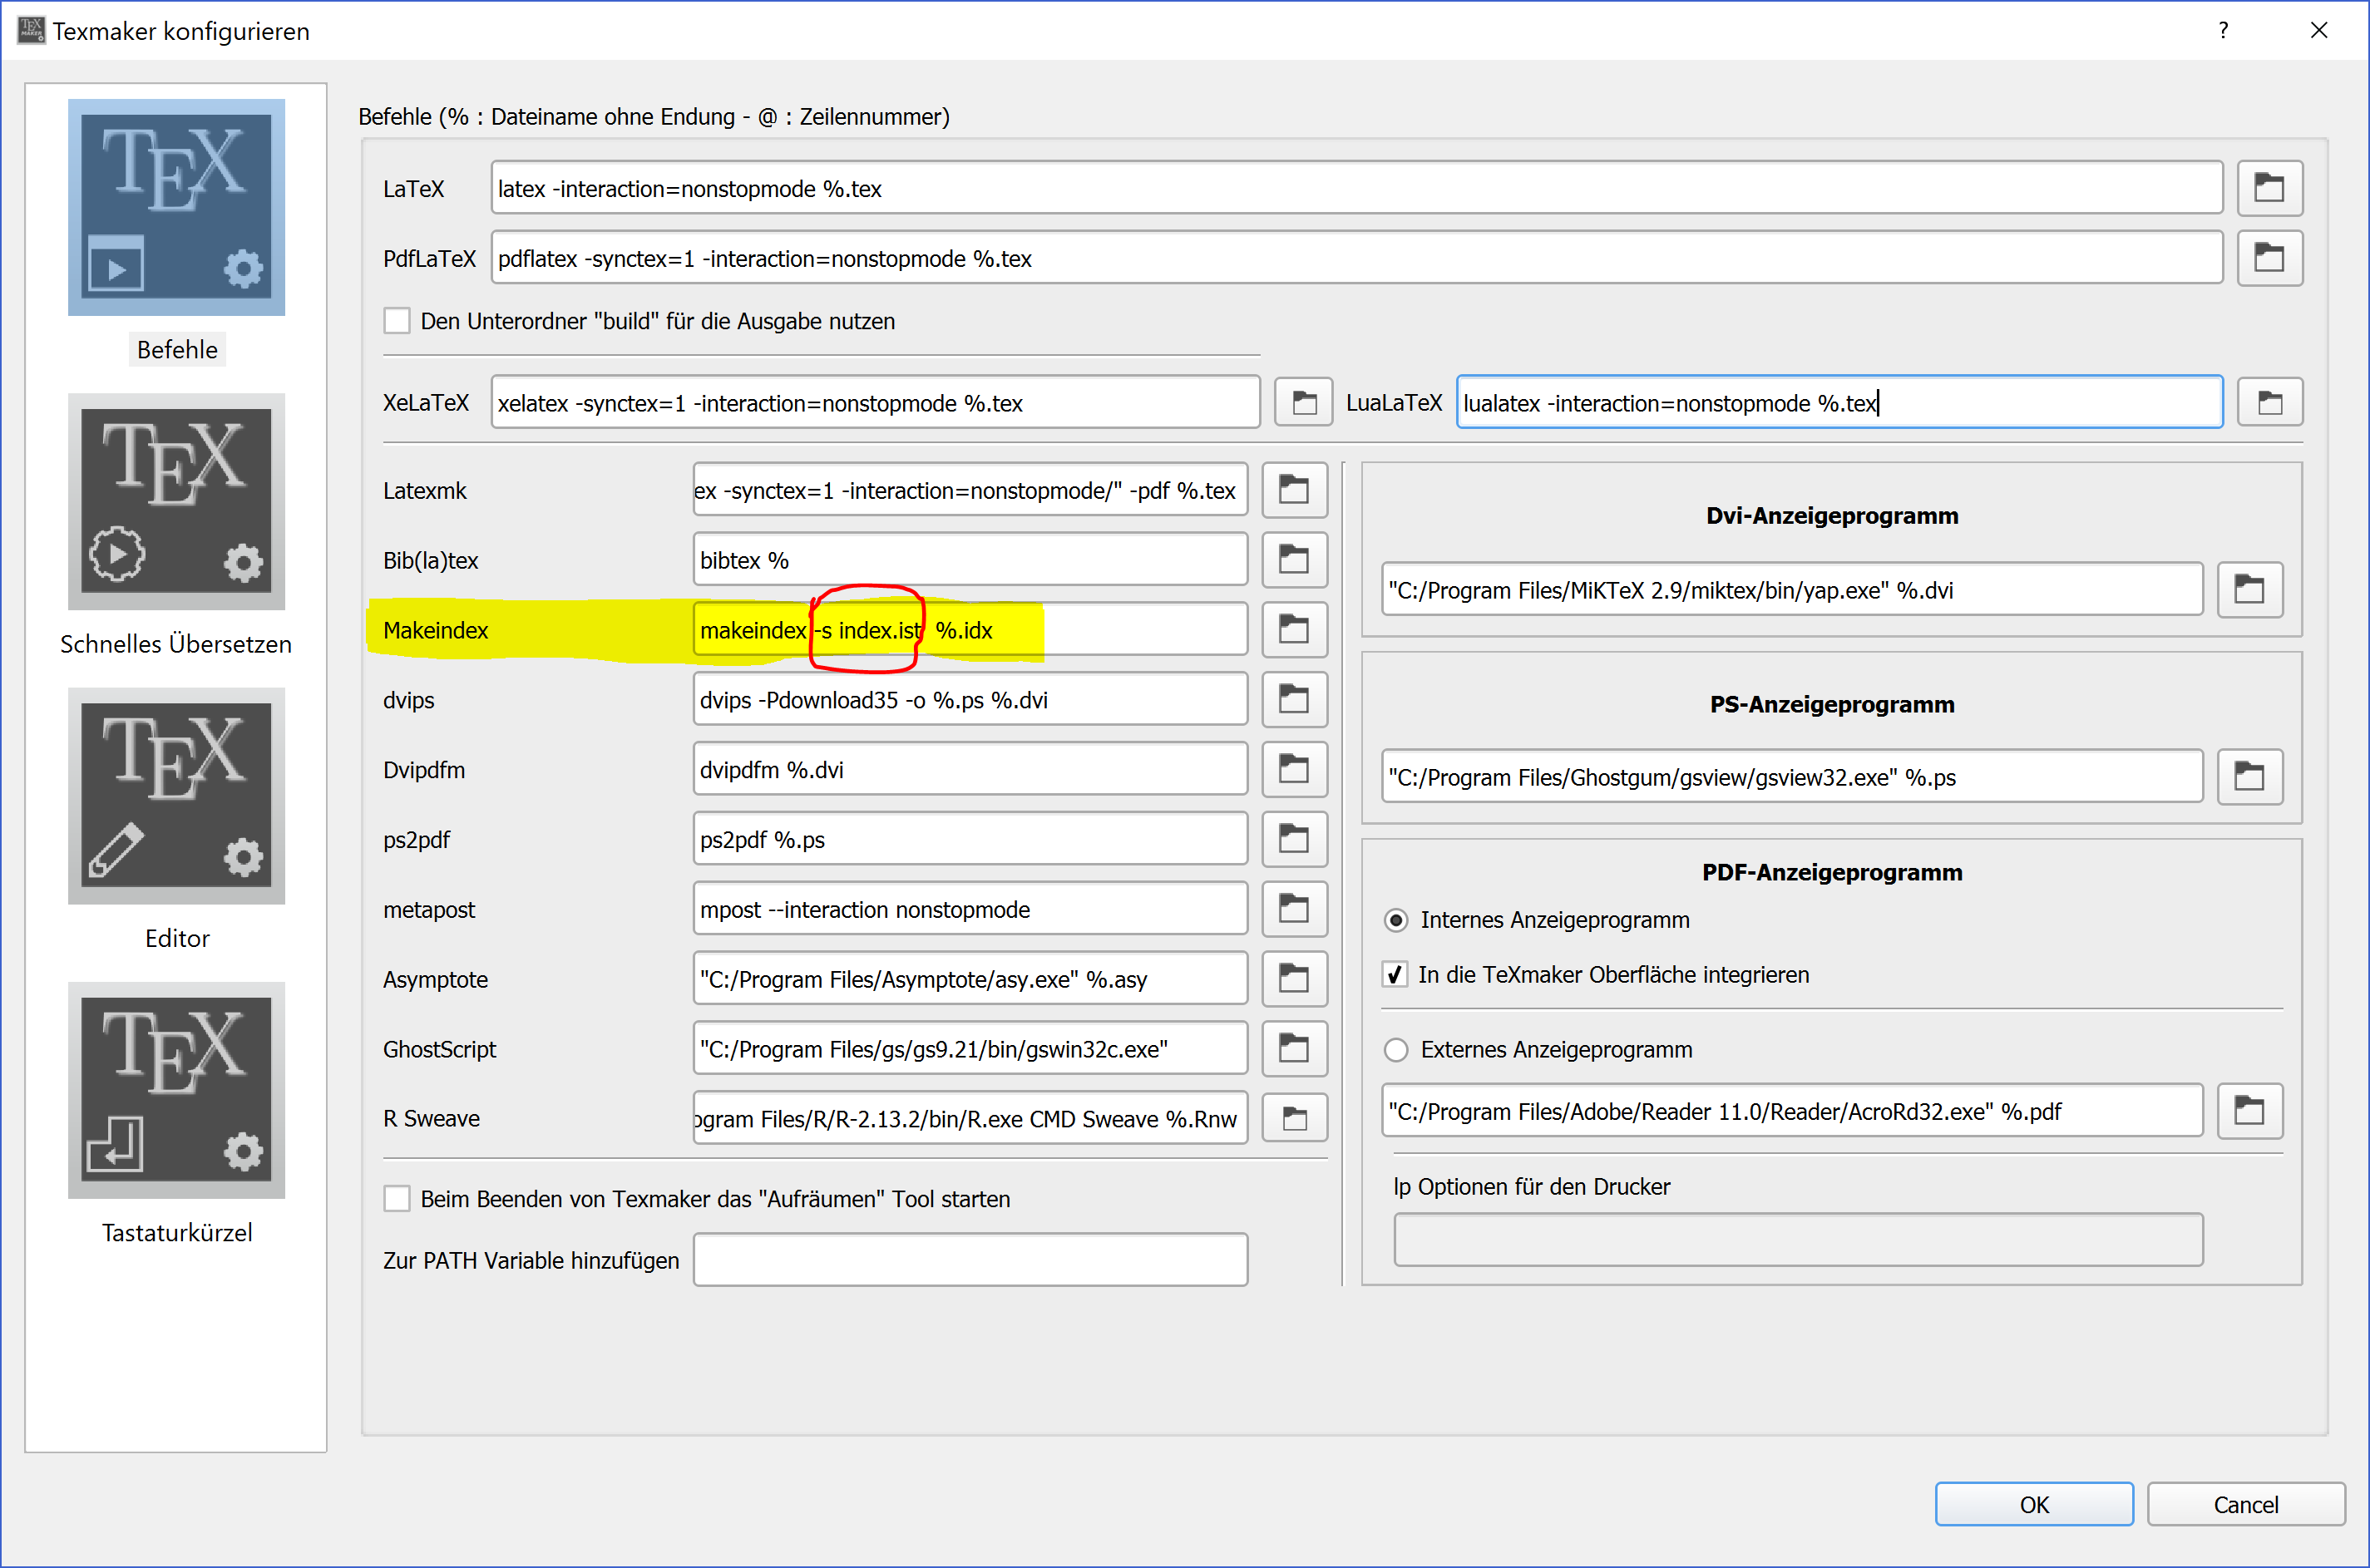
\includegraphics[width=0.6\textwidth]{./Bilder/Texmaker_Konfiguration_1.PNG}
  \caption{Konfiguration Latex: Befehle}
  \label{fig:Konfig}
\end{figure}

\begin{figure}[h!]
\centering
  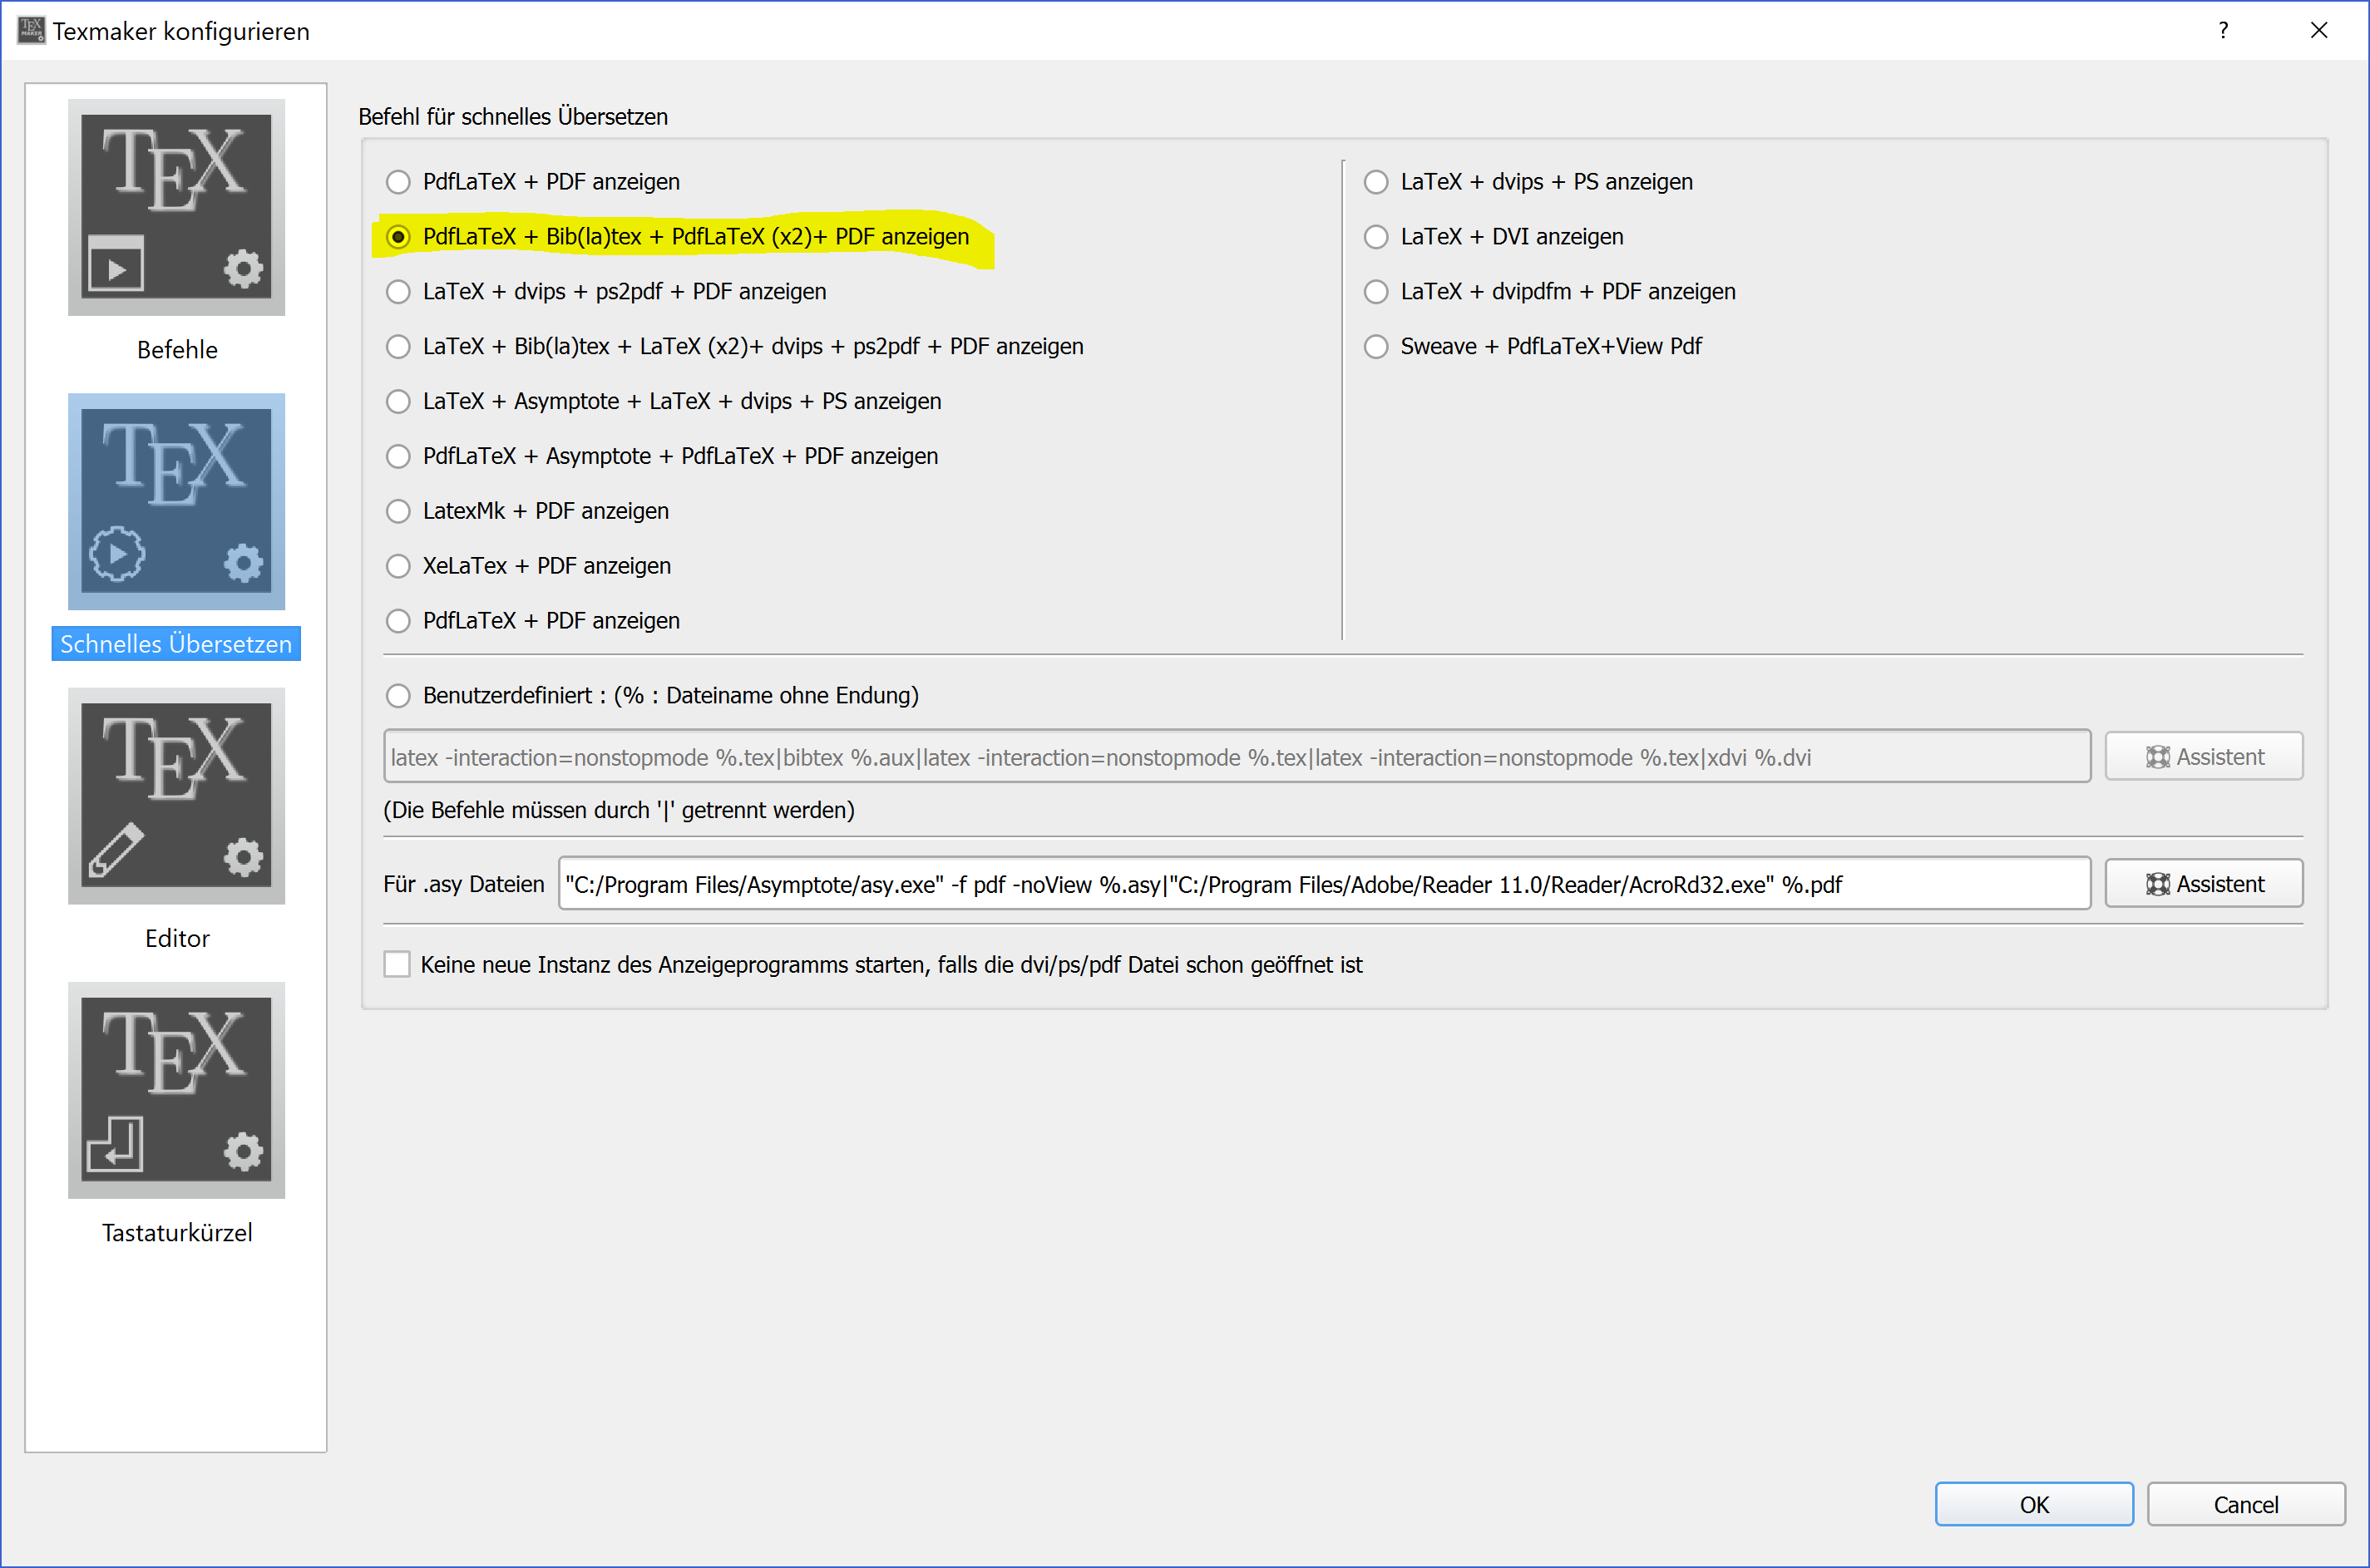
\includegraphics[width=0.6\textwidth]{./Bilder/Texmaker_Konfiguration_2.PNG}
  \caption{Konfiguration Latex: Schnelles Übersetzen}
\end{figure}

Zusätzlich muss dass Stichwortverzeichnis mit \keys{F12} manuell erstellt werden.

\textbf{\\Empfehlung:} 
\begin{quote}
Mit der Tasten-Folge \keys{F1} \keys{F12} \keys{F1} wird alles korrekt erstellt.
\end{quote}

\end{spacing}
%
%
%
%
%
% ===== Kapitel 2 ======
%
\pagebreak 
\section{Trennung von Inhalt und Struktur} 
\begin{spacing}{1.25}
Dieses \LaTeX\ Tutorial / Template ist so aufgebaut, dass die Struktur-Informationen des zu erstellenden Dokumentes in der Haupt-Datei *.tex abgelegt ist. Alle Inhalte des Dokumentes sind in verschiedenen Verzeichnissen in weiteren Dateien enthalten.

\begin{figure}[h!]
\centering
  % 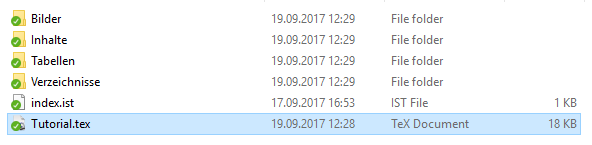
\includegraphics[width=0.75\textwidth]{./Bilder/VerzeichnisStruktur.PNG}      % Bild ohne Rahmen
  \fbox{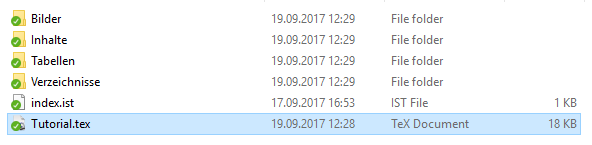
\includegraphics[width=0.75\textwidth]{./Bilder/VerzeichnisStruktur.PNG}} % Bild mit Rahmen
  \caption{Die Verzeichnis-Struktur des Dokumentes}
\end{figure}

Die Datei \menu{Tutorial.tex} ist das Kerndokument. Diese Datei ethält die Struktur (Reihenfolge der Kapitel) des Dokumentes, sowie alle benötigten Befehle für die Formatierung und für die Erstellung der verschiedenen zu generierenden Verzeichnisse (wie z.B. das Inhaltsverzeichnis, das Stichwortverzeichnis, etc.).  

Die Datei \menu{index.ist} enthält die Style-In\-for\-ma\-ti\-on\-en zum Stichwortverzeichnis. Dies wäre nicht zwingend notwendig. Da mir aber das Layout des von LaTeX automatisch erstellten Stichwortverzeichnisses nicht gefällt, habe ich dieses mit dieser Style-Datei angepasst. Dies muss in der Konfiguration von Texmaker entpsrechend angegeben werden (siehe auch \cref{fig:Konfig}: \nameref{fig:Konfig} auf Seite \pageref{fig:Konfig}).

Sämtliche (fachlichen) Inhalte des Dokumentes werden in separaten Dokumenten innerhalb der jeweiligen Verzeichnisse (Bilder, Inhalte, Tabellen, Verzeichnisse) abgelegt. Diese werden als einfache Text-Dateien mit Endung \menu{*.tex} erfasst. 

Auf den folgenden Seiten dieses Tutorials wird gezeigt, wie Text erfasst und in Absätze gegliedert wird, mit welchen Befehlen man Bilder und Grafiken einbinden kann, wie Tabellen erstellt werden, wie Querverweise innerhalb des Dokumentes erstellt werden, wie korrekt mit Abkürzungen gearbeitet wird, wie Begriffe in das Stichwortverzeichnis aufgenommen werden und wie Fussnoten sowie Literatur- / Quellenangaben erfasst  und gesetzt werden.

Dieses Tutorial / Template selbst verwendet alle im Inhaltsverzeichis aufgeführten Punkte \& Inhalte. Damit kann der Source-Text dieses Tutorials / Template \menu{Tutorial.tex} ebenfalls als Quelle für die Beantwortung vieler Fragen genommmen werden.

\end{spacing}
%
%
%
%
%
% ===== Kapitel 3 ======
%
\pagebreak 
\section{Formale Vorgaben abholen / beachten} 
\begin{spacing}{1.25}
Arbeiten heisst immer auch dokumentieren. Projekt-, Produkt-, System-, Benutzer-Do\-ku\-men\-ta\-ti\-on\-en oder spätestens beim Abschluss der Berufslehre die IPA - das Erstellen von Dokumentationen ist (Berufs-) Alltag. Deshalb erhältst Du im Lehrlabor verschiedentlich die Aufgabe, eine schriftliche (technische, wissenschaftliche) Dokumentation zu verfassen.

Bevor nun mit der eigentlichen (fachlichen) Dokumentation begonnen wird:

\begin{quote}
    \begin{tcolorbox} 
        Vergewissere Dich unbedingt vor dem Beginn Deiner Arbeit bei Deiner Betreuungsperson, 
        ob sich die äussere Form (Formatierung, Layout, Reihenfolge der Kapitel, etc.) dieses
        Dokumentes mit den Vorgaben deckt, bzw. hole unbedingt bei Deiner Betreuungsperson ab, 
        an welche Richtlinien / Vorgaben Du Dich für Deine Dokumentation halten musst. 
    \end{tcolorbox}
\end{quote}

Das Template ist so aufgebaut, dass Anpassungen vorgenommen werden können, ohne sehr tiefe \LaTeX -Kenntnisse zu benötigen. Die Verwendung dieses Templates sollte somit keine Kopfschmerzen verursachen.  

\end{spacing}
%
%
%
%
%
% ===== Kapitel 4 ======
%
\pagebreak 
\section{Text erfassen} 
\begin{spacing}{1.25}
Dieses Tutorial / Template ist so aufgebaut, dass in der Datei \menu{Tutorial.tex} alle Struktur-Informationen des Dokumentes enthalten sind. Im wesentlichen sind dies die Reihenfolge aller Kapitel (section) und Unterkapitel (subsection).

\begin{figure}[h!]
\centering
  % 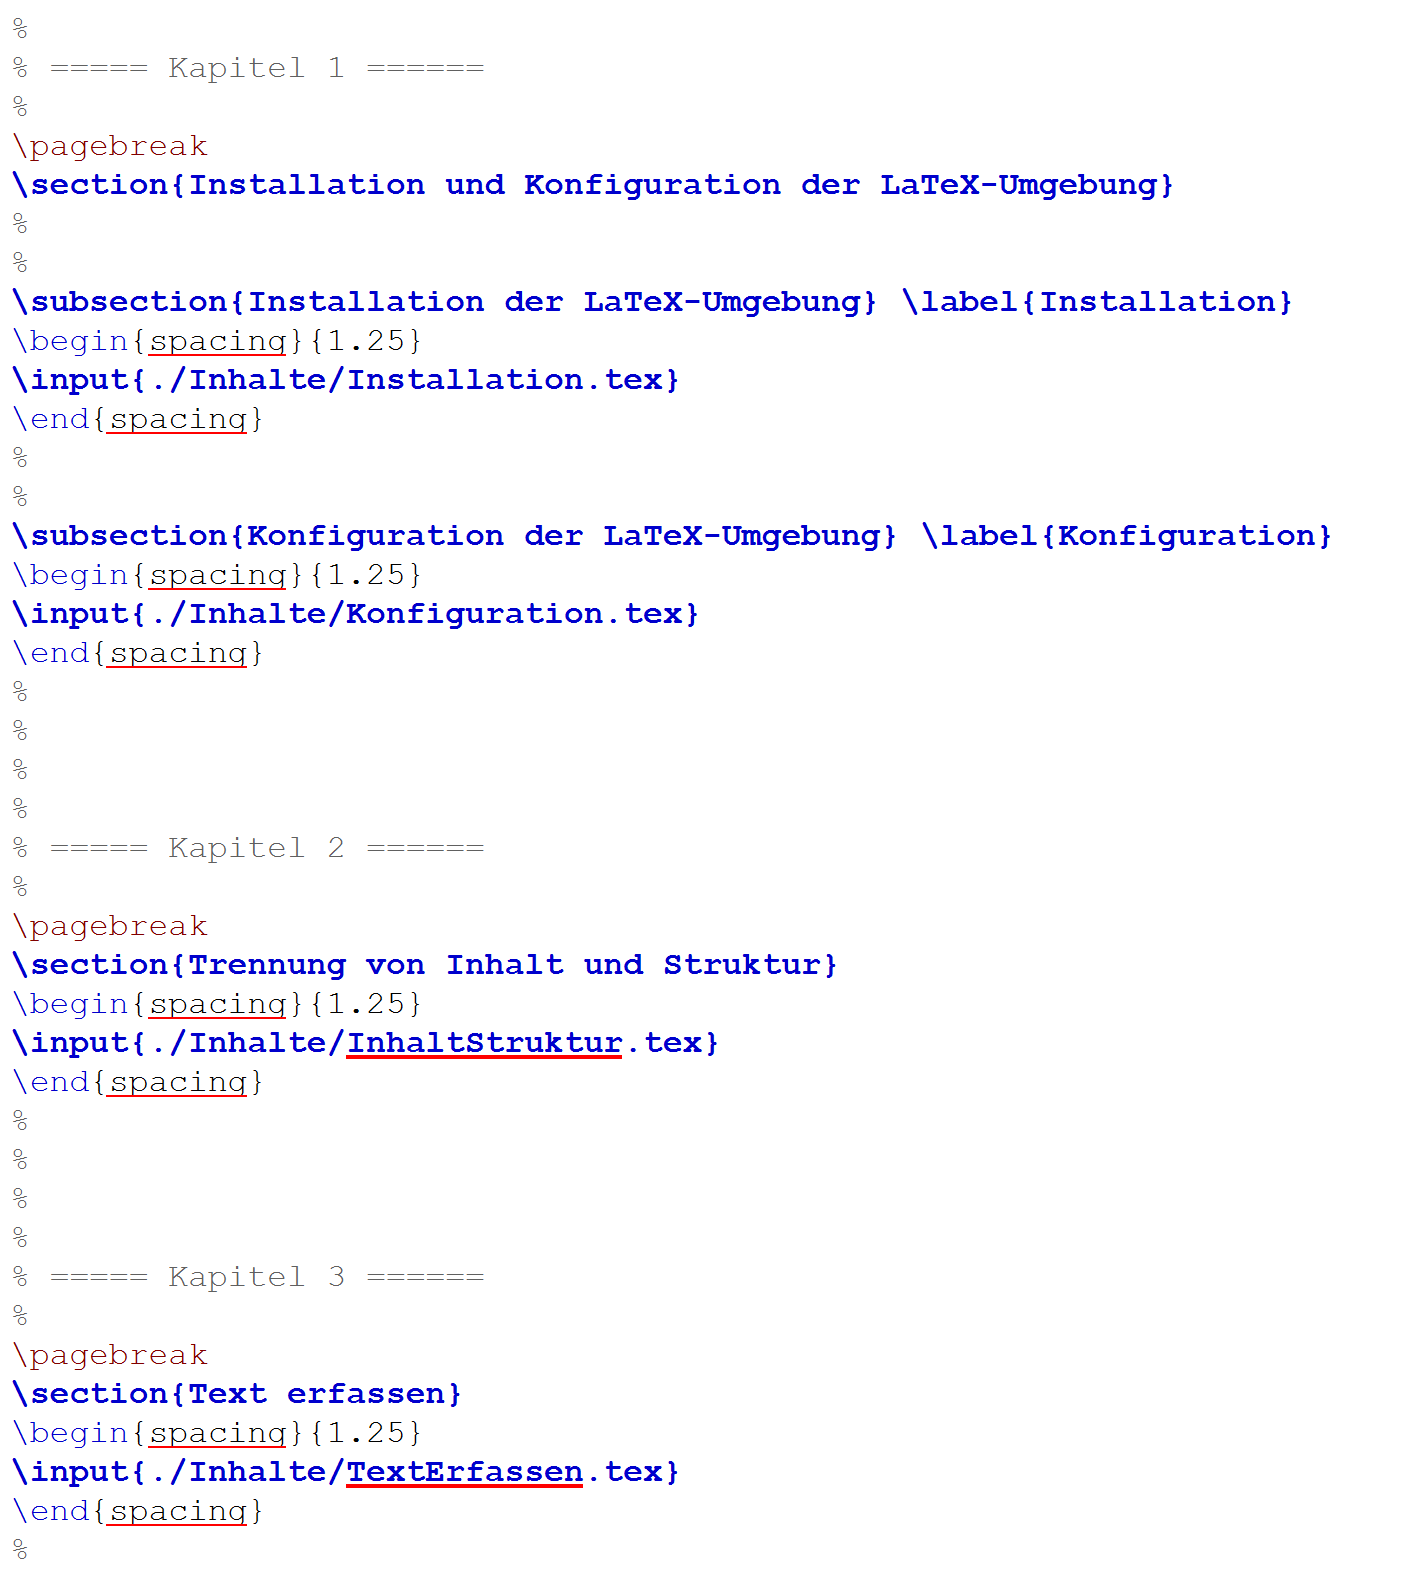
\includegraphics[width=0.9\textwidth]{./Bilder/TextStruktur_1.png}        % Bild ohne Rahmen
  \fbox{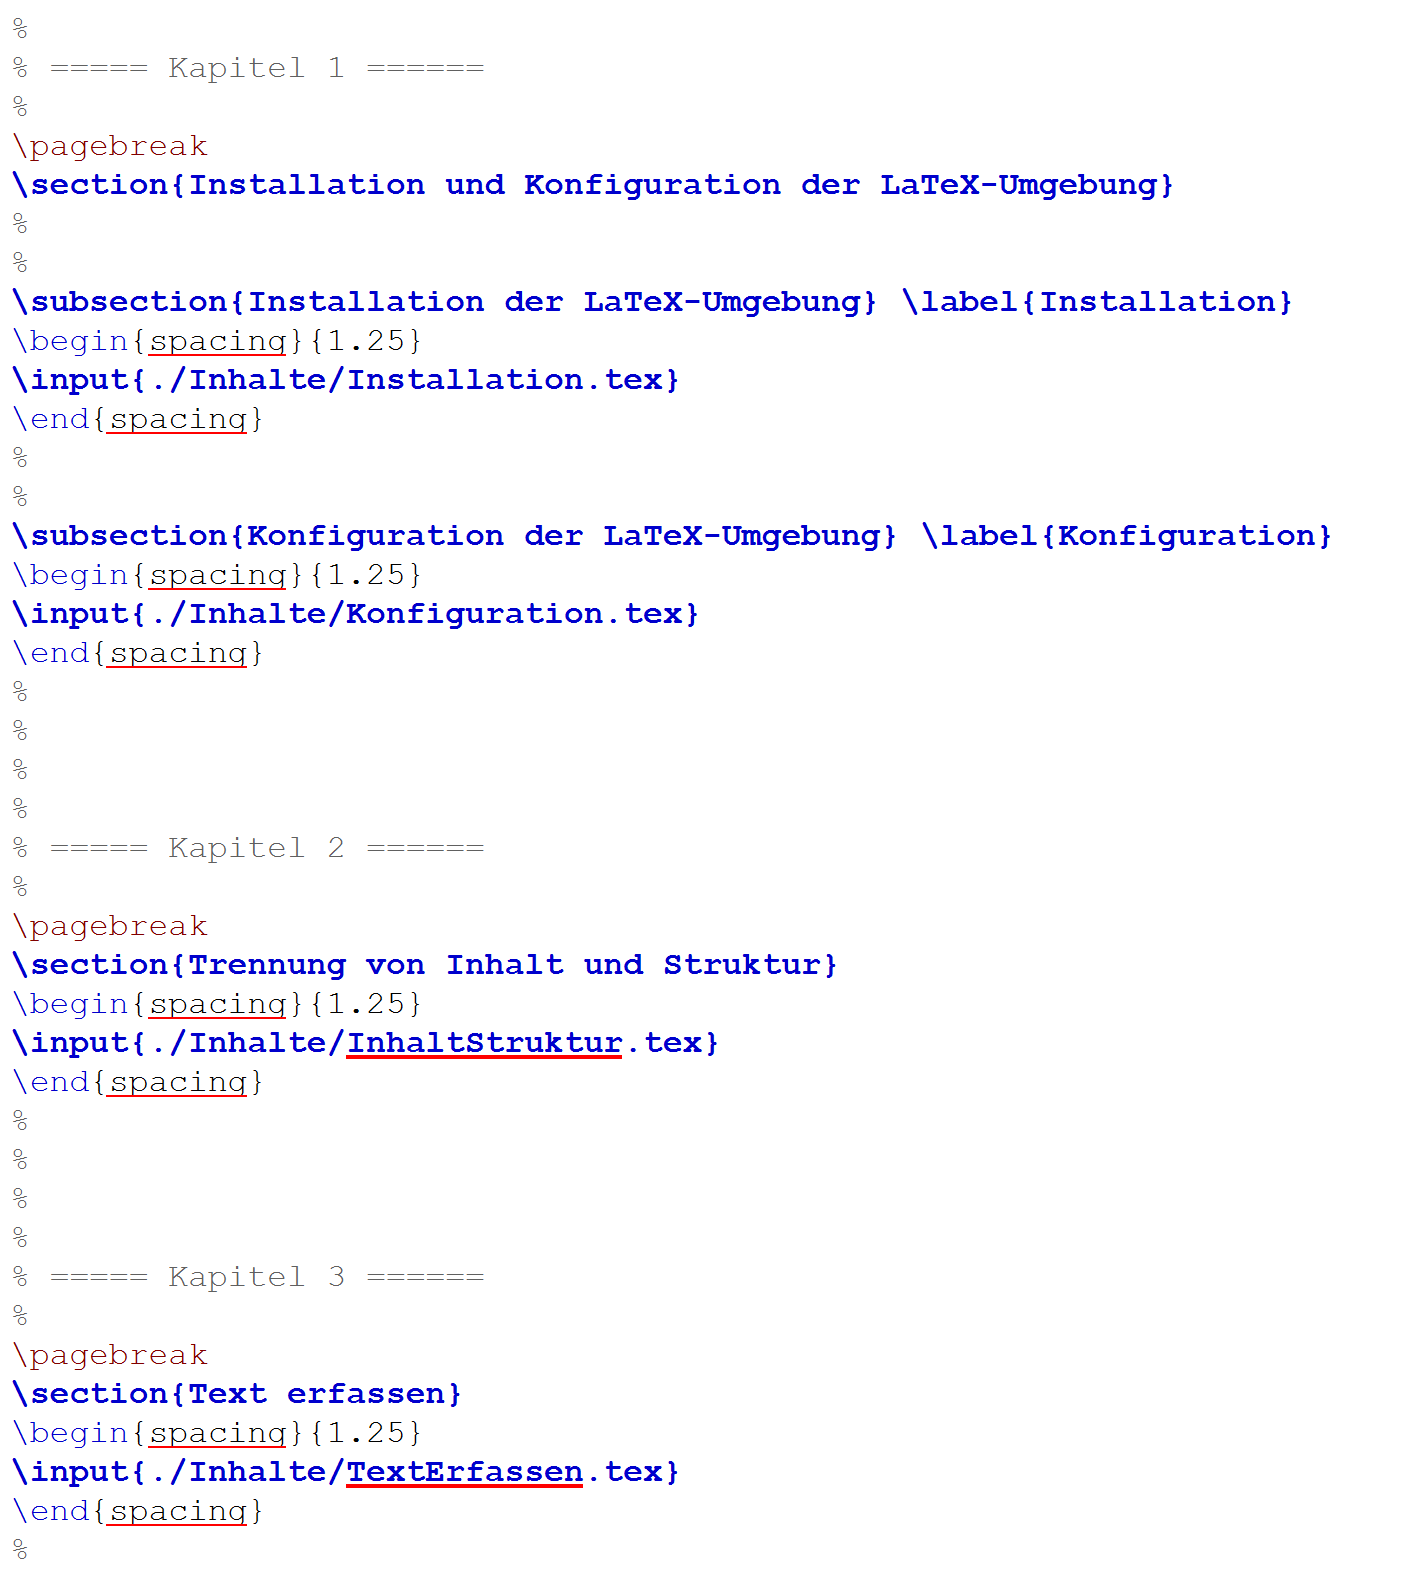
\includegraphics[width=0.9\textwidth]{./Bilder/TextStruktur_1.png}}   % Bild mit Rahmen
  \caption{Kapitel-Struktur des Dokumentes}
  \label{fig:KapitelStruktur}
\end{figure} 

Die eigentlichen fachlichen (Text-) Inhalte der Kapitel sind in separaten \menu{*.tex} Dateien im Verzeichnis \menu{Inhalte} erfasst, die mit dem Befehl \code{\textbackslash{input\{...\}}} eingebunden / eingefügt werden (siehe \cref{fig:KapitelStruktur}: \nameref{fig:KapitelStruktur} auf Seite \pageref{fig:KapitelStruktur}).

\end{spacing}
%
%
\subsection{Text formatieren}
\label{TextFormatieren}
\begin{spacing}{1.25}
An dieser Stelle sollen exemplarische einige Beispiele gezeigt werden, wie in \LaTeX\ Texte \textbf{Fett}, \textcolor{red}{farbig}, \textit{Kursiv}, \underline{unterstrichen}, \uuline{doppelt unterstrichen}, \uwave{unterschlängelt}, \sout{horizontal durchgestrichen}, \xout{schräg durchgestrichen} gesetzt werden und wie Texte formatiert / struk\-tu\-riert werden können.

Ebenso soll gezeigt werden, wie obige Beispiel-Aufzählung 

\begin{itemize}[topsep=0em, partopsep=0em, parsep=0em, itemsep=0em]
	\item \textbf{Fett}, 
	\item \textcolor{red}{farbig}, 
	\item \textit{Kursiv}, 
	\item \underline{unterstrichen}, 
	\item \uuline{doppelt unterstrichen}, 
	\item \uwave{unterschlängelt}, 
	\item \sout{horizontal durchgestrichen}, 
	\item \xout{schräg durchgestrichen},
\end{itemize}

auch als Liste gesetzt werden kann und wie ein selber definiertes Aufzählungszeichen 

\begin{itemize}[leftmargin=9em, topsep=0em, partopsep=0em, parsep=0em, itemsep=0em]
	\item[--]                 \textbf{Fett}, 
	\item[-]                  \textcolor{red}{farbig}, 
	\item[*]                  \textit{Kursiv}, 
	\item[\textgreater]       \underline{unterstrichen}, 
	\item[+]                  \uuline{doppelt unterstrichen}, 
	\item[zum Ersten:]        \uwave{unterschlängelt}, 
	\item[zum Zweiten:]       \sout{horizontal durchgestrichen}, 
	\item[als letztes noch:]  \xout{schräg durchgestrichen},
\end{itemize}

gesetzt werden kann.

\end{spacing}
%
%
\subsubsection{Gliederung / Strukturierung}
\begin{spacing}{1.25}

Wie Eingangs dieses Kapitels erwähnt, ist dieses Template so vorbereitet, dass die Gliederung / Strukturierung des Inhaltes in Kapitel (section), Unterkapitel (subsection) und Unterunterkapitel (subsubsection) im Haupt-Dokument gemacht wird. Aus dem Haupt-Dokument werden dann die Inhalte der einzelnen  Kapitel (section), Unterkapitel (subsection) und Unterunterkapitel (subsubsection) referenziert (siehe \cref{fig:KapitelStruktur}: \nameref{fig:KapitelStruktur} auf Seite \pageref{fig:KapitelStruktur}).

Sollen tiefere Kapitel-Strukturen als Unter-Unter-Kapitel verwendet werden, so ist dies zwar möglich, bedeutet aber einiges an Aufwand, da dies nicht mit den \LaTeX\ Standardmitteln gemacht werden kann. Dies ist ein bewusster Entscheid von Leslie Lamport\footnote{Leslie Lamport auf Wikipedia: \url{https://de.wikipedia.org/wiki/Leslie_Lamport}} - das La in \LaTeX\ steht für Lamport\cite{Lamport2017}. 

\begin{quote}
    \begin{tcolorbox} 
        LaTeX’s set of \dq sections\dq{} stops at the level of \code{\textbackslash{subsubsection}}.
        This reflects a design decision by Lamport — for, after all, 
        who can reasonably want a section with such huge strings of 
        numbers in front of it\cite{Tex2017}? 
    \end{tcolorbox}
\end{quote}

Somit bleibt für die Gliederung / Strukturierung der referenzierten Dokumente nur noch die Gliederung / Strukturierung in sogenannte Absätze. Es wäre technisch zwar möglich, auch in den aus dem Haupt-Dokument referenzierten Dokumenten Kapitel und Unterkapitel zu definieren. Davon rate ich jedoch dringend ab, da die Übersicht damit garantiert verloren geht und die am Ende resultierende tatsächliche Gliederung / Strukturierung eher ein Zufallsprodukt als wirklich unter Kontrolle ist. 

In den Inhalts-Dokumenten wollen wir also nur fachlichen Inhalt, keine Kapitel Strukturierung. Es können weitere Dateien eingebunden werden. Dabei beschränken wir uns jedoch auf inhaltliche Elemente wie Grafiken und Tabellen.

\end{spacing}
%
%
\subsubsection{Absätze}
\begin{spacing}{1.25}

Folgendes Beispiel zeigt, wie Absätze erfasst werden:

\begin{figure}[h!]
    \centering
      % 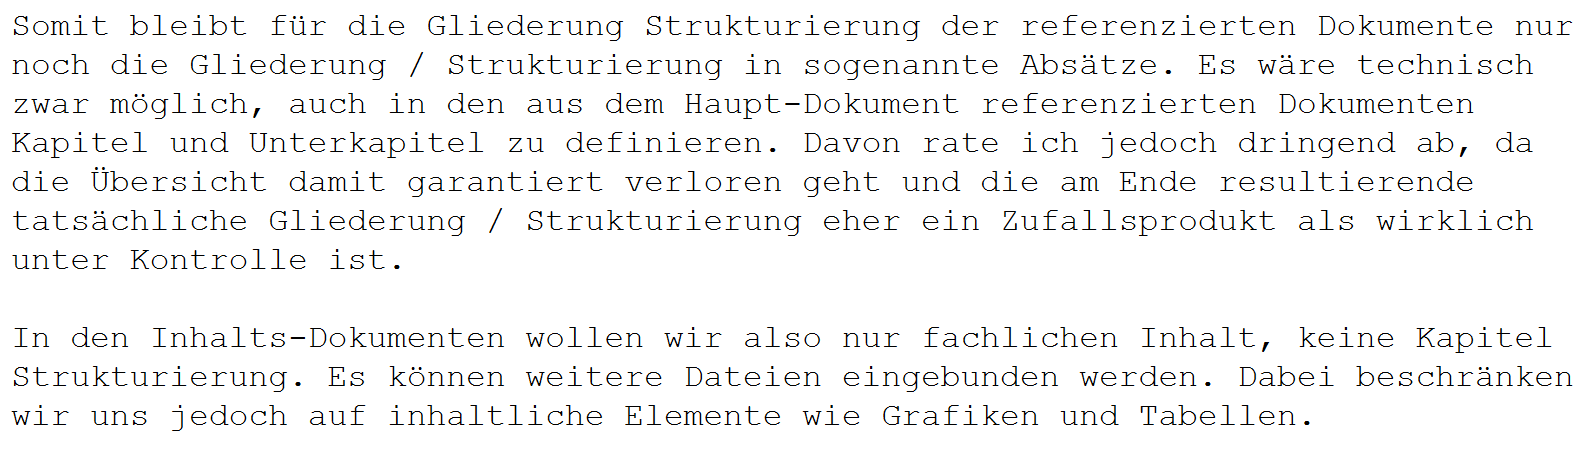
\includegraphics[width=0.85\textwidth]{./Bilder/GliederungAbsatz.png}        % Bild ohne Rahmen
      \fbox{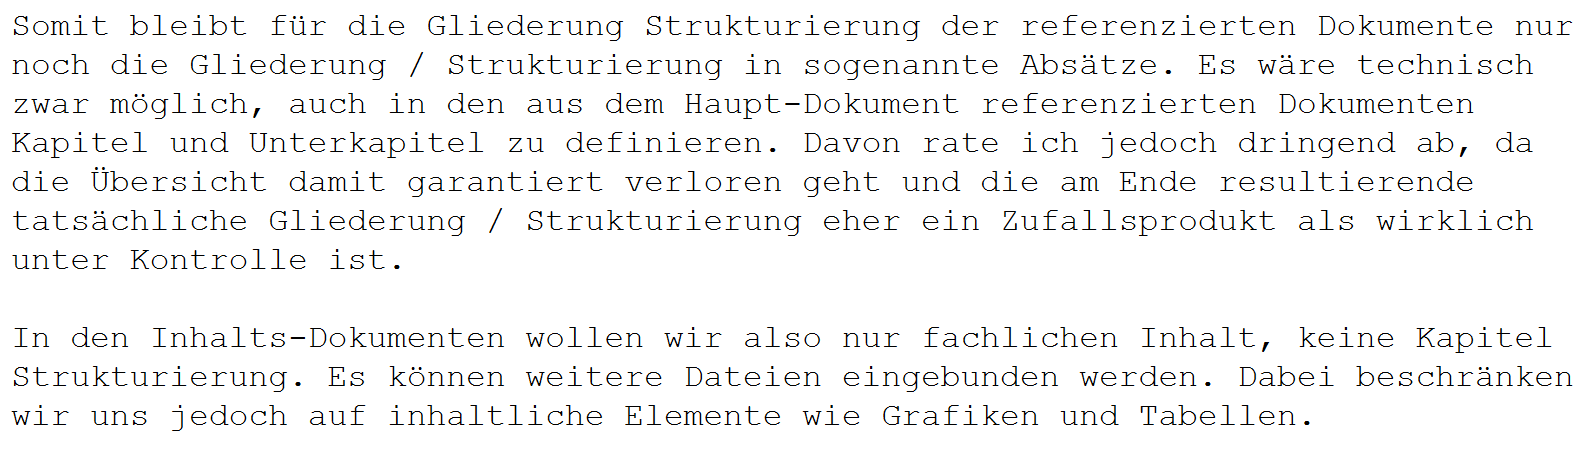
\includegraphics[width=0.85\textwidth]{./Bilder/GliederungAbsatz.png}}   % Bild mit Rahmen
      \caption{Absätze im Dokument}
    \label{fig:GliederungAbsatz}
\end{figure} 

Ein neuer Absatz wird durch eine Leerzeile im Text erzeugt. Die Anzahl der Leerzeilen und die Anzahl der Leerzeichen zwischen einzelnen Wörtern spielen keine Rolle. \LaTeX\ formatiert den (Fliess-) Text innerhalb eines Absatzes selber. Einfluss darauf wird über spezielle \LaTeX\ -Befehle genommen, die in folgenden Kapiteln behandelt werden.
 
\end{spacing}
%
%
\subsubsection{Schriftarten und Farben}
\begin{spacing}{1.25}
Für die bereits Eingangs dieses Kapitels gezeigten Schriftarten und Farben:

\begin{quote}

An dieser Stelle sollen exemplarische einige Beispiele gezeigt werden, wie in \LaTeX\ Texte \textbf{Fett}, \textcolor{red}{farbig}, \textit{Kursiv}, \underline{unterstrichen}, \uuline{doppelt unterstrichen}, \uwave{unter\-schlängelt}, \sout{horizontal durchgestrichen}, \xout{schräg durchgestrichen} gesetzt werden und wie Texte formatiert / struk\-tu\-riert werden können.

\end{quote}

ist folgender \LaTeX-Code notwendig: 

\begin{figure}[h!]
    \centering
      \fbox{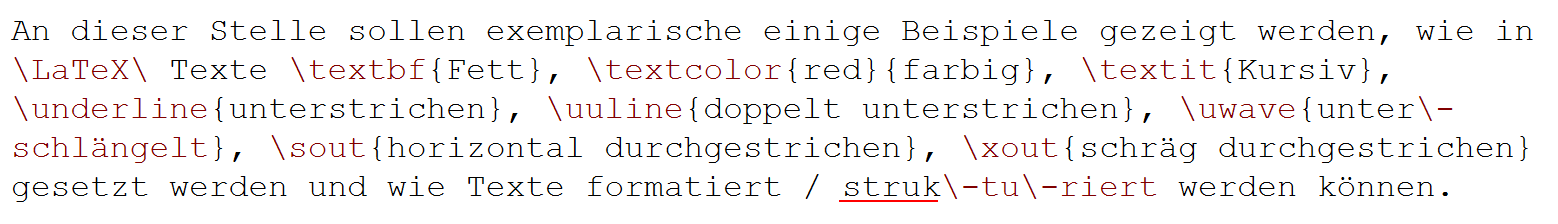
\includegraphics[width=0.75\textwidth]{./Bilder/TextArtenFarben.png}}  
      \caption{Schriftarten und Farben}
\end{figure} 

In diesem Beispiel sieht man auch, wie \LaTeX\ die korrekte Trennung von Wörtern mitgeben kann (siehe die Worte unterschlängelt und strukturiert).

\end{spacing}
%
%
\subsubsection{Aufzählungen \& Bullet-Points}
\begin{spacing}{1.25}

Für die ebenfalls Eingangs dieses Kapitels gezeigte Aufzählung mit den Standard Auf\-zählungs\-zeichen, ist folgende Code notwendig:

\begin{figure}[h!]
    \centering
      \fbox{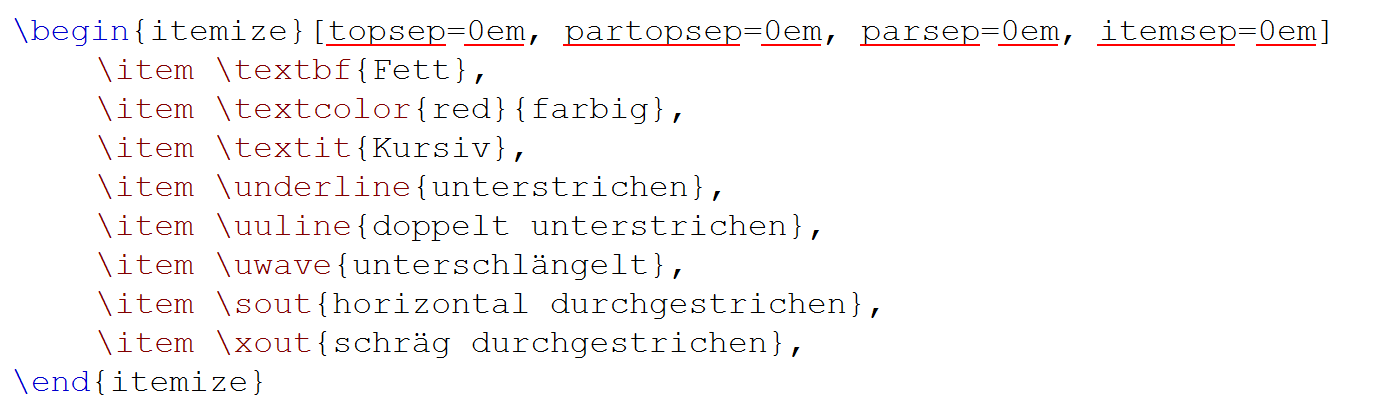
\includegraphics[width=0.75\textwidth]{./Bilder/TextBulletPointsStandard.png}}  
      \caption{Eigene Aufzählungszeichen}
\end{figure} 

Über die verschiedenen Seperatoren in der ersten Zeile, können die Abstände zwischen den einzelnen Aufzählungspunkten eingestellt werden. 


Die mit diesem Code erzeugte Aufzählung ist auf Seite \pageref{TextFormatieren} zu sehen.

\newpage Für Aufzählung mit selber definierten Aufzählungszeichen, ist folgende Code notwendig:

\begin{figure}[h!]
    \centering
      \fbox{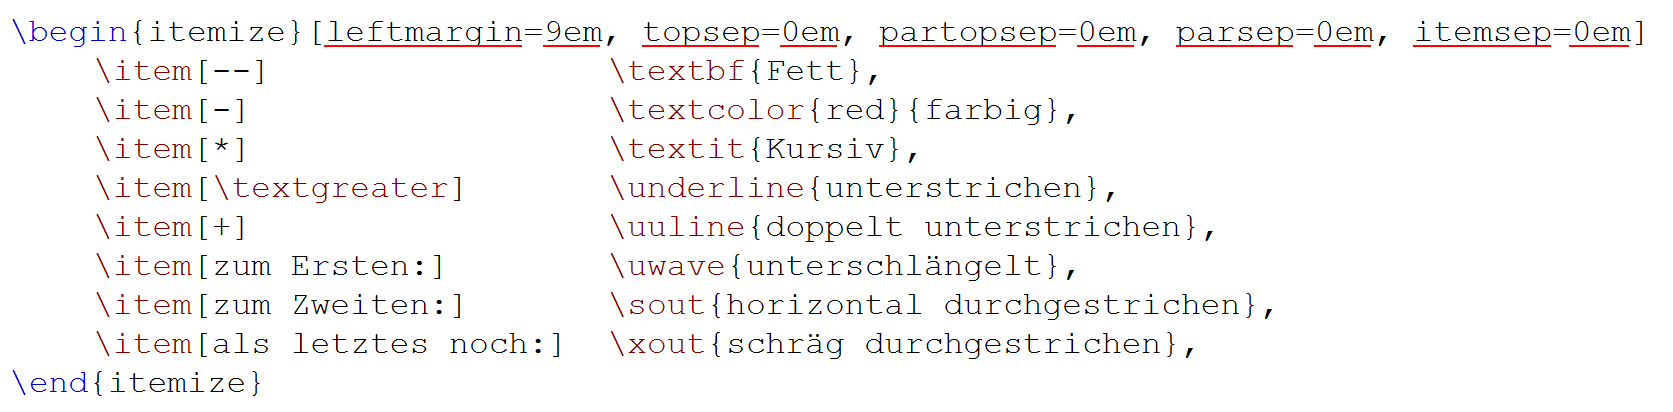
\includegraphics[width=0.75\textwidth]{./Bilder/TextBulletPoints.png}}  
      \caption{Eigene Aufzählungszeichen}
\end{figure} 

Auch hier werden über die verschiedenen Seperatoren in der ersten Zeile die Abstände zwischen den einzelnen Aufzählungspunkten eingestellt. Da in diesem Beispiel jedoch 'sehr lange' Aufzählungszeichen (z.B. 'als letztes noch') verwendet werden, muss die ganze Aufzählung deutlich mehr eingerückt werden (leftmargin=9em).  
 
Auch die mit diesem Code erzeugte Aufzählung ist auf Seite \pageref{TextFormatieren} zu sehen.

Dieses Beispiel zeigt, dass die Anzahl der Leerzeichen zwischen Worten resp, zwischen dem Aufzählungszeichen und den Worten keine Rolle spielt, da \LaTeX\ die Formatierung selber vornimmt.

\end{spacing}
%
%
%
%
% ===== Kapitel 5 ======
%
\pagebreak 
\section{Arbeiten mit Tabellen}
\begin{spacing}{1.25}
In diesem Kapitel werden einige Beispiele zu Tabellen gezeigt. Um die Darstellung von Tabellen besser zeigen zu können, ist jede Tabelle in einer eigenen Datei definiert, die mit \code{\textbackslash{input\{tabellenDatei.tex\}}} eingebunden wird.

\textbf{Hinweis:} In vielen LaTeX-Editoren (u.a. auch in Texmaker) gibt es Kommandos oder Makros für die Erstellung von Tabellen. Ebenfalls gibt es Online Generatoren für LaTeX Tabellen\footnote{\url{http://www.tablesgenerator.com/}}. 

\end{spacing}
%
%
\subsection{Tabellen ohne Schraffierung}
\begin{spacing}{1.25}
Tabellen sind in Latex nicht ganz einfach zu verwalten. Die hier gezeigten Beispiele sollten jedoch vielen Anforderungen genügen. Für kompliziertere Tabellen empfehle ich Google und Youtube, wo sehr viele Tutorials zur Verfügung stehen.

Starten wir mit einem einfachen Beispiel:


\begin{table}[h!]
\begin{center}
\begin{tabular}{|c|c|c|}
\hline
Spalte 1         &     Spalte 2           &     Spalte 3             \\
\hline
Zelle 1.1        &     Zelle 1.2          &     Zelle 1.3            \\
\hline
Zelle zwei.eins  &     Zelle zwei.zwei    &     Zelle zwei.drei      \\
\hline
\end{tabular}
\caption{Eine erste LaTeX-Tabelle}
\end{center}
\end{table}



Der für diese Tabelle verwendete Code sieht wie folgt aus:

\begin{figure}[h!]
    \centering
      \fbox{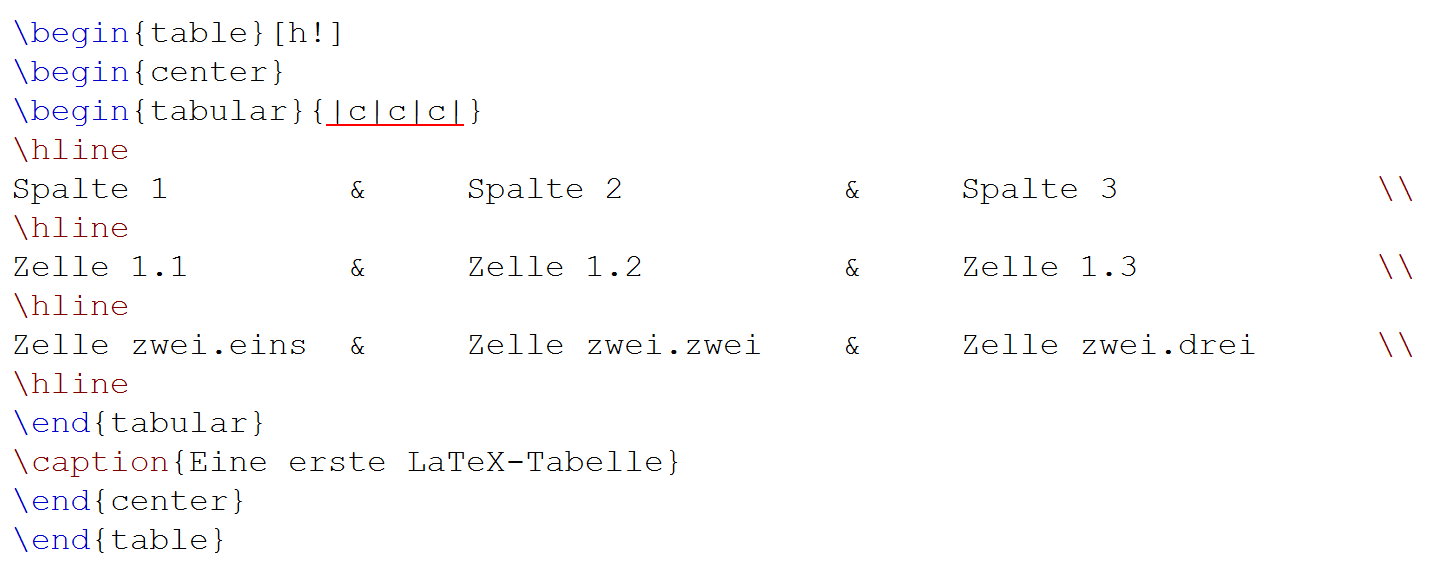
\includegraphics[width=0.75\textwidth]{./Bilder/Tabelle_1.png}}  
      \caption{Eine erste LaTeX-Tabelle}
\end{figure} 

Die Spalten richten sich nach deren Inhalt aus und sind zentriert (c) ausgerichtet, unabhängig davon, wie die einzelnen Spalten in der \code{*.tex}-Datei formatiert sind. 

In folgender Tabelle wollen wir die Spaltenbreite und die Spaltenausrichtung selber kontrollieren. Das Ergebnis sieht wie folgt aus:   


\begin{table}[h!]
\begin{center}
\begin{tabular}{p{4.5cm}|C{3.5cm}|R{4.5cm}}
Spalte 1              &   Spalte 2            &   Spalte 3                \\ 
\hline
Linksbündig           &   Zentriert           &   Rechtsbündig            \\  
\hline
linksbündige Spalte   &   zentrierte Spalte   &   rechtsbündige Spalte    \\ 
\end{tabular}
\caption{Eine zweite LaTeX-Tabelle}
\end{center}
\end{table}



Der dazu benötigte Code:

\begin{figure}[h!]
    \centering
      \fbox{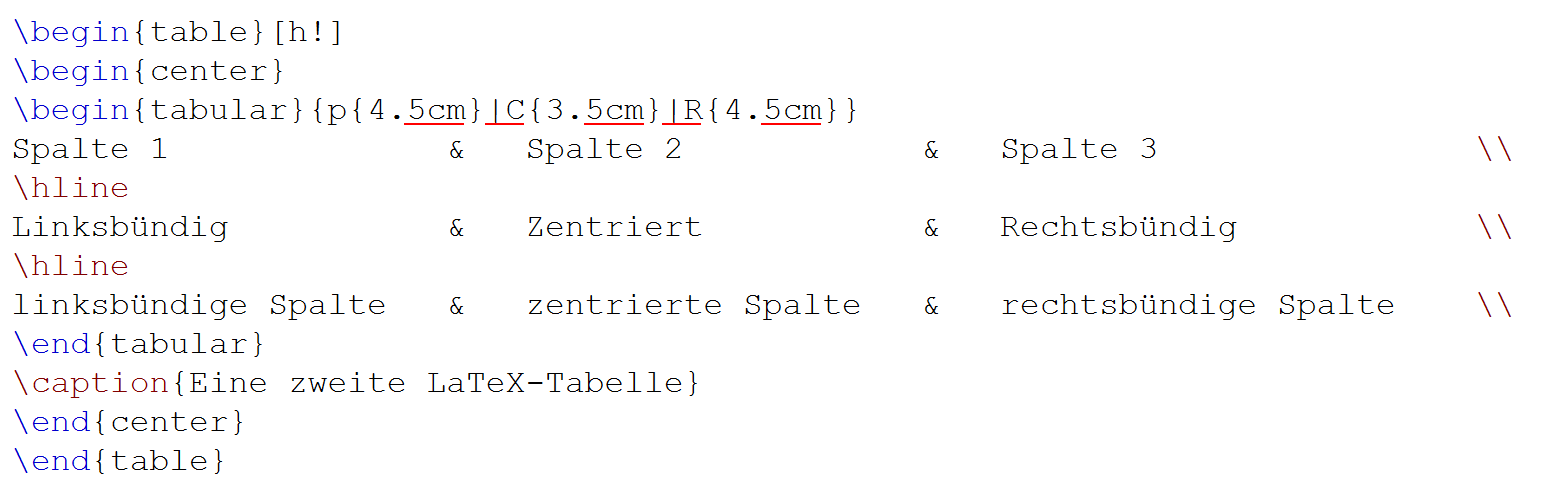
\includegraphics[width=0.75\textwidth]{./Bilder/Tabelle_2.png}}  
      \caption{Eine zweite LaTeX-Tabelle}
\end{figure} 

Der hier gezeigte Code funktioniert nur, wenn in der Präambel die hier verwendeten Befehle eigenhändig definiert werden.

\begin{figure}[h!]
    \centering
      \fbox{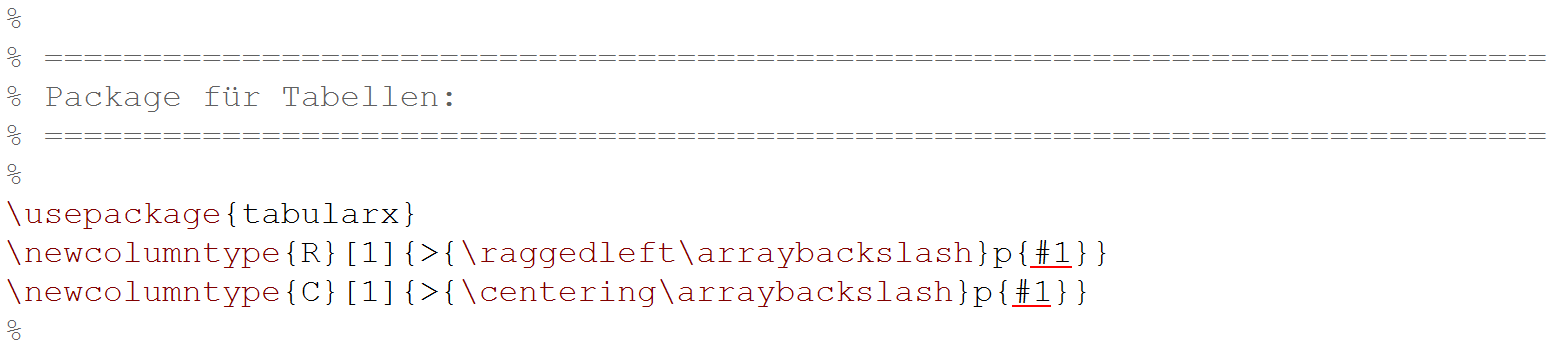
\includegraphics[width=0.75\textwidth]{./Bilder/Tabelle_Praeambel.png}}  
      \caption{LaTeX-Tabellen Präambel}
\end{figure} 

Hier noch ein Beispiel mit verschiedenen Schriftarten in den Zellen und anderen Linien für die Separierung der Zeilen.


\begin{table}[h!]
\begin{center}
\begin{tabular}{p{2cm} C{2cm} R{2cm}}
\toprule
\textbf{Wer}    &    Wo     &    \textit{Was}     \\ 
\midrule
\textbf{ich}    &    da     &    \textit{dies}    \\  
\textbf{du}     &    hier   &    \text{das}       \\ 
\bottomrule
\end{tabular}
\caption{Eine dritte LaTeX-Tabelle}
\end{center}
\end{table}



\newpage
Der hierfür benötigte Code:

\begin{figure}[h!]
    \centering
      \fbox{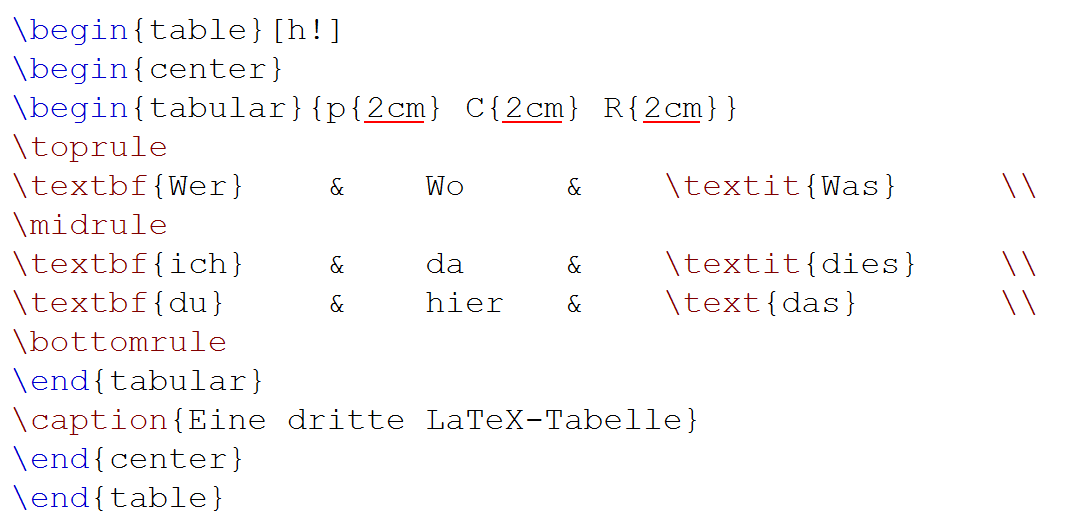
\includegraphics[width=0.75\textwidth]{./Bilder/Tabelle_3.png}}  
      \caption{Eine dritte LaTeX-Tabelle}
\end{figure} 

\end{spacing}
%
%
\subsection{Tabellen mit Schraffierung}
\begin{spacing}{1.25}
In den nächsten Beispielen wird gezeigt, wie Spalten resp. Zeilen eingefärbt werden:  


\begin{table}[h!]
\begin{center}
\begin{tabular}{l|c|c|c}
          & Spalte 1                      &     Spalte 2                 &      Spalte 3                   \\
\hline
Zeile 1   & \cellcolor{gray!50}Zelle 1.1 & \cellcolor{gray!50}Zelle 1.2  & \cellcolor{gray!50}Zelle 1.3    \\
\hline
Zeile 2   & Zelle 2.1                    & Zelle 2.2                     & Zelle 2.3 \\
\hline
Zeile 3   & \cellcolor{gray!50}Zelle 3.1 & \cellcolor{gray!50}Zelle 3.2  & \cellcolor{gray!50}Zelle 3.3    \\
\hline
Zeile 4   & Zelle 4.1                    & Zelle 4.2                     & Zelle 4.3 \\
\hline
Zeile 5   & \cellcolor{gray!50}Zelle 5.1 & \cellcolor{gray!50}Zelle 5.2  & \cellcolor{gray!50}Zelle 5.3    \\
\hline
Zeile 6   & Zelle 6.1                    & Zelle 6.2                     & Zelle 6.3                       \\
\end{tabular}
\caption{Eine vierte LaTeX-Tabelle}
\end{center}
\end{table}



\begin{figure}[h!]
    \centering
      \fbox{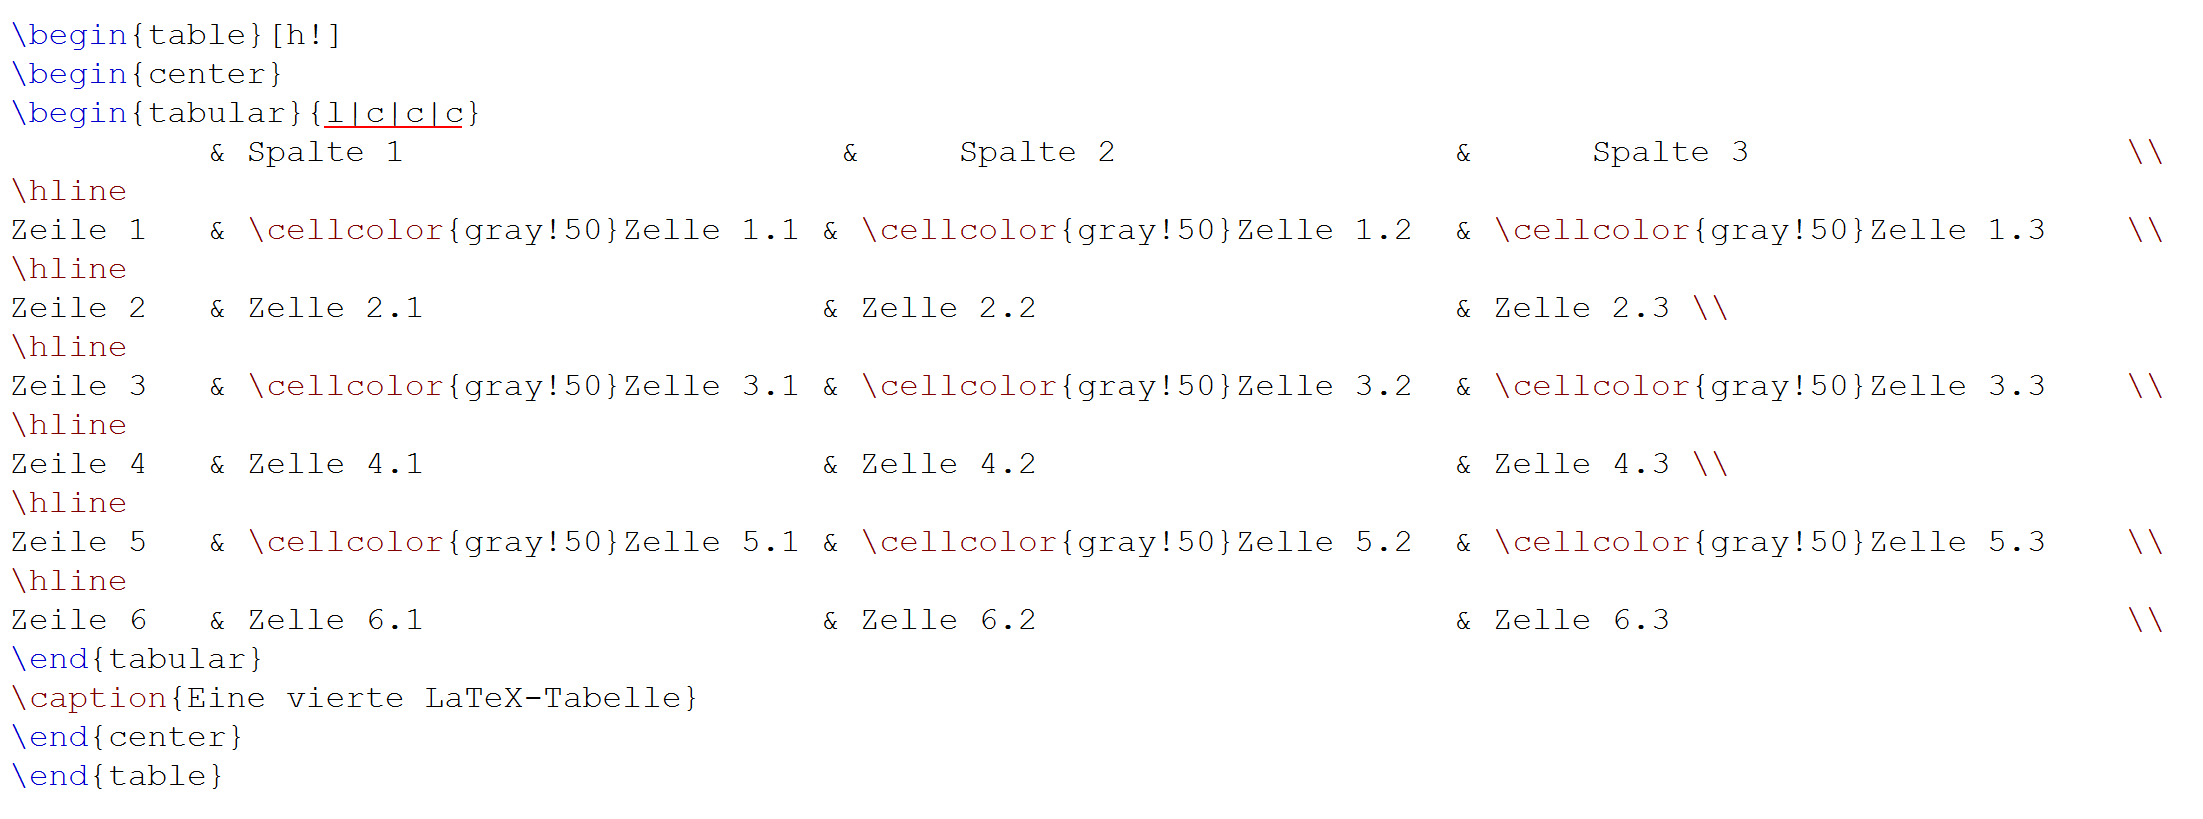
\includegraphics[width=0.75\textwidth]{./Bilder/Tabelle_4.png}}  
      \caption{Eine vierte LaTeX-Tabelle}
\end{figure} 

\newpage
Ein zweites Beispiel:


\begin{table}[h!]
\begin{center}
\begin{tabular}{p{1.5cm}|p{2.5cm}|p{2.5cm}|p{2.5cm}}
                   & \textbf{Spalte 1}              & \textbf{Spalte 2} & \textbf{Spalte 3}              \\
\hline
\textbf{Zeile 1}   & \cellcolor{gray!50}Zelle 1.1   & Zelle 1.2         & \cellcolor{gray!50}Zelle 1.3   \\
\hline
\textbf{Zeile 2}   & \cellcolor{gray!50}Zelle 2.1   & Zelle 2.2         & \cellcolor{gray!50}Zelle 2.3   \\
\hline
\textbf{Zeile 3}   & \cellcolor{gray!50}Zelle 3.1   & Zelle 3.2         & \cellcolor{gray!50}Zelle 3.3   \\
\hline
\textbf{Zeile 4}   & \cellcolor{gray!50}Zelle 4.1   & Zelle 4.2         & \cellcolor{gray!50}Zelle 4.3   \\
\hline
\textbf{Zeile 5}   & \cellcolor{gray!50}Zelle 5.1   & Zelle 5.2         & \cellcolor{gray!50}Zelle 5.3   \\
\hline
\textbf{Zeile 6}   & \cellcolor{gray!50}Zelle 6.1   & Zelle 6.2         & \cellcolor{gray!50}Zelle 6.3   \\
\end{tabular}
\caption{Eine fünfte LaTeX-Tabelle}
\end{center}
\end{table}



\begin{figure}[h!]
    \centering
      \fbox{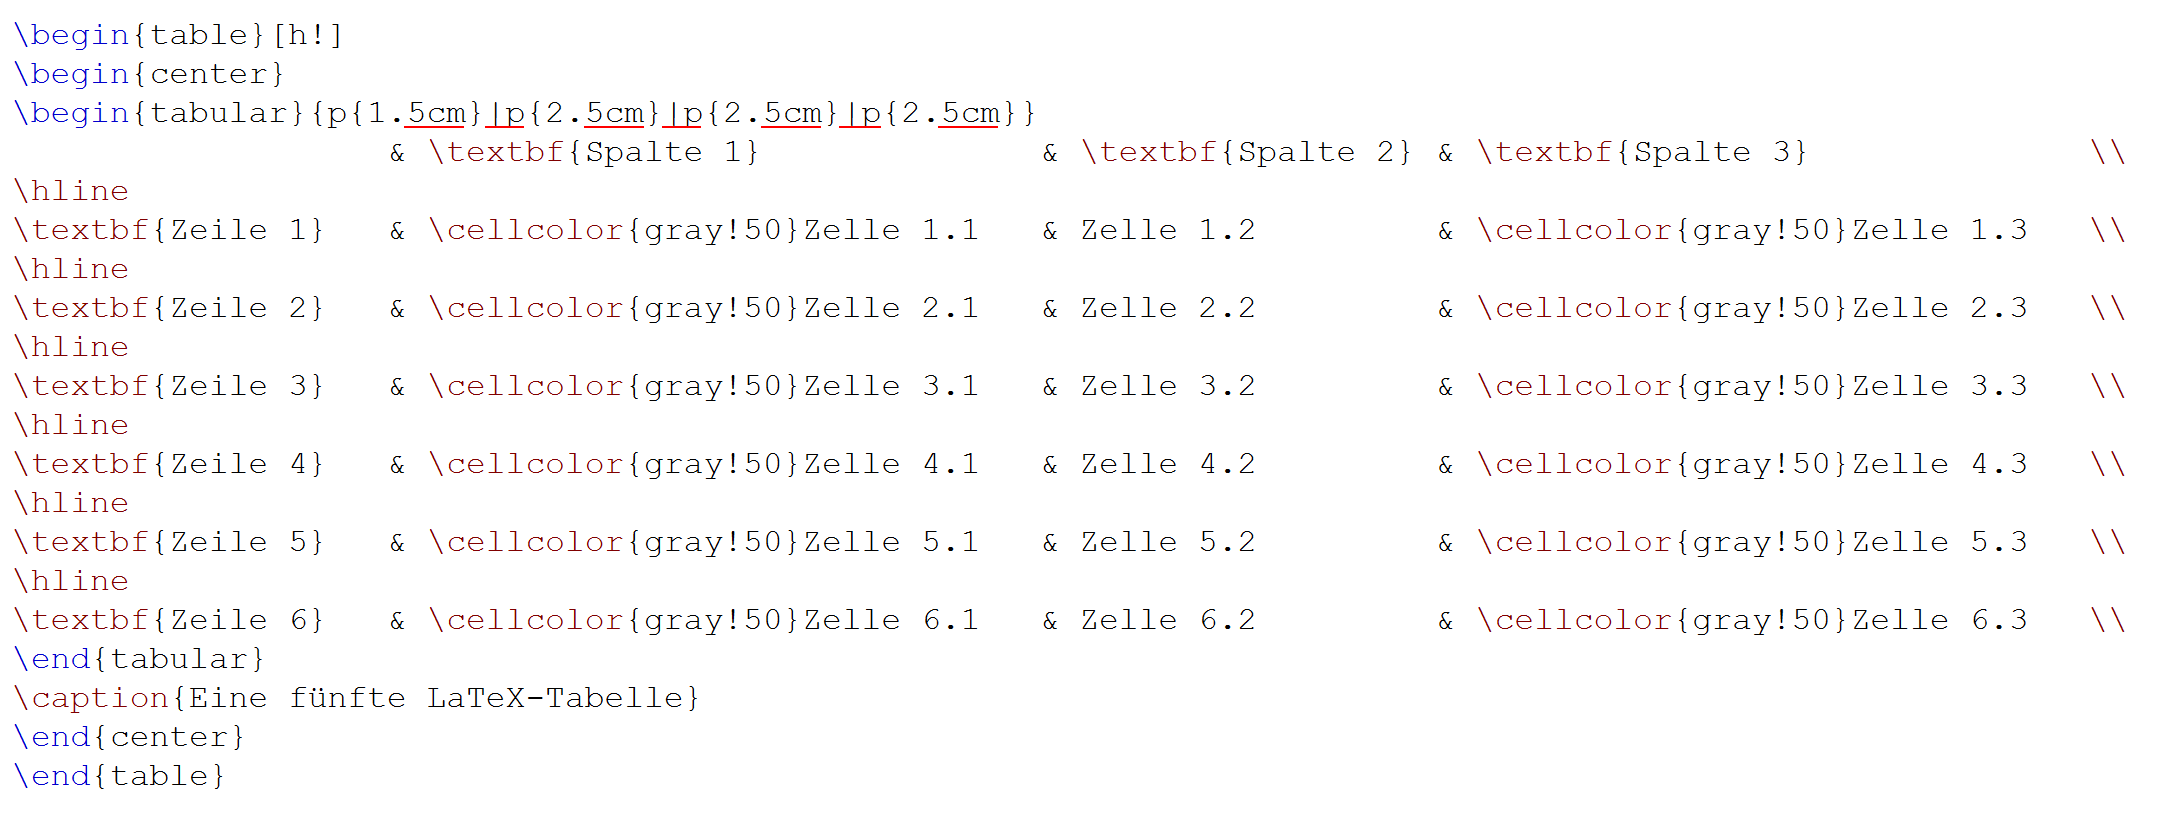
\includegraphics[width=0.7\textwidth]{./Bilder/Tabelle_5.png}}  
      \caption{Eine fünfte LaTeX-Tabelle}
\end{figure} 

Ein drittes Beispiel:


\begin{table}[h!]
\begin{center}
\begin{tabular}{c|c|c}
\rowcolor{gray!50} Spalte 1      &   Spalte 2     &   Spalte 3     \\
\hline
Zelle 1.1                        &   Zelle 1.2    &   Zelle 1.3    \\
\hline
Zelle 2.1                        &   Zelle 2.2    &   Zelle 2.3    \\
\end{tabular}
\caption{Eine sechste LaTeX-Tabelle}
\end{center}
\end{table}



\begin{figure}[h!]
    \centering
      \fbox{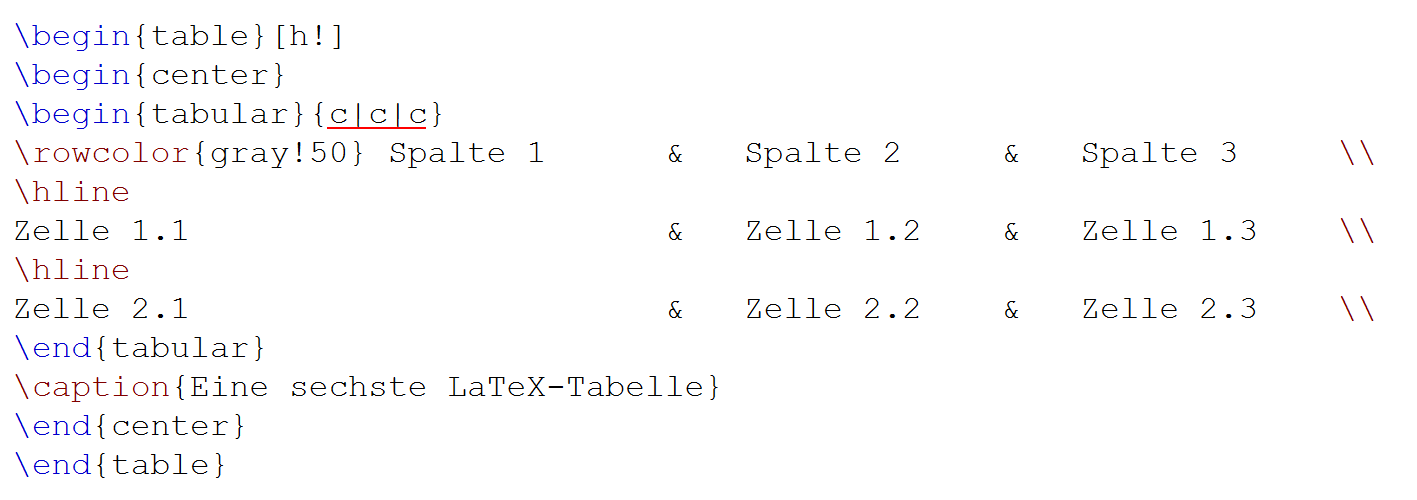
\includegraphics[width=0.7\textwidth]{./Bilder/Tabelle_6.png}}  
      \caption{Eine sechste LaTeX-Tabelle}
\end{figure} 

\textbf{Wichtig:} Die Formatierung der Tabellen in den \code{*.tex}-Dateien dient lediglich der Übersicht, resp. der Lesbarkeit des Codes für den Autor.

\end{spacing}
%
%
%
%
%
% ===== Kapitel 6 ======
%
\pagebreak 
\section{Arbeiten mit Bildern / Grafiken}
\begin{spacing}{1.25}
In diesem Kapitel wird eine speziellere Variante der Platzierung von Bildern und Grafiken auf einer Seite gezeigt. Das Einbinden / Anzeigen von einzelnen Bildern ist in den vorhergehenden Kapiteln mehrfach zu sehen.

\vfill

Der \LaTeX-Löwe einmal mit und einmal ohne Rahmen, nebeneinander platziert. 

\begin{figure}[htb]
    \centering
    \begin{minipage}[t]{0.45\linewidth}
        \centering
        
\includegraphics[width=0.9\linewidth]{./Bilder/LaTeX.jpg}
        \caption{\LaTeX-Löwe ohne Rahmen}
    \end{minipage}
    \hfill
    \begin{minipage}[t]{0.45\linewidth}
        \centering
        \fbox{
\includegraphics[width=0.9\linewidth]{./Bilder/LaTeX.jpg}}
        \caption{\LaTeX-Löwe mit Rahmen}
    \end{minipage}
\end{figure}

\vfill

Der \LaTeX-Code für die Platzierung der beiden \LaTeX-Löwen nebeneinander:

\begin{figure}[h!]
    \centering
      \fbox{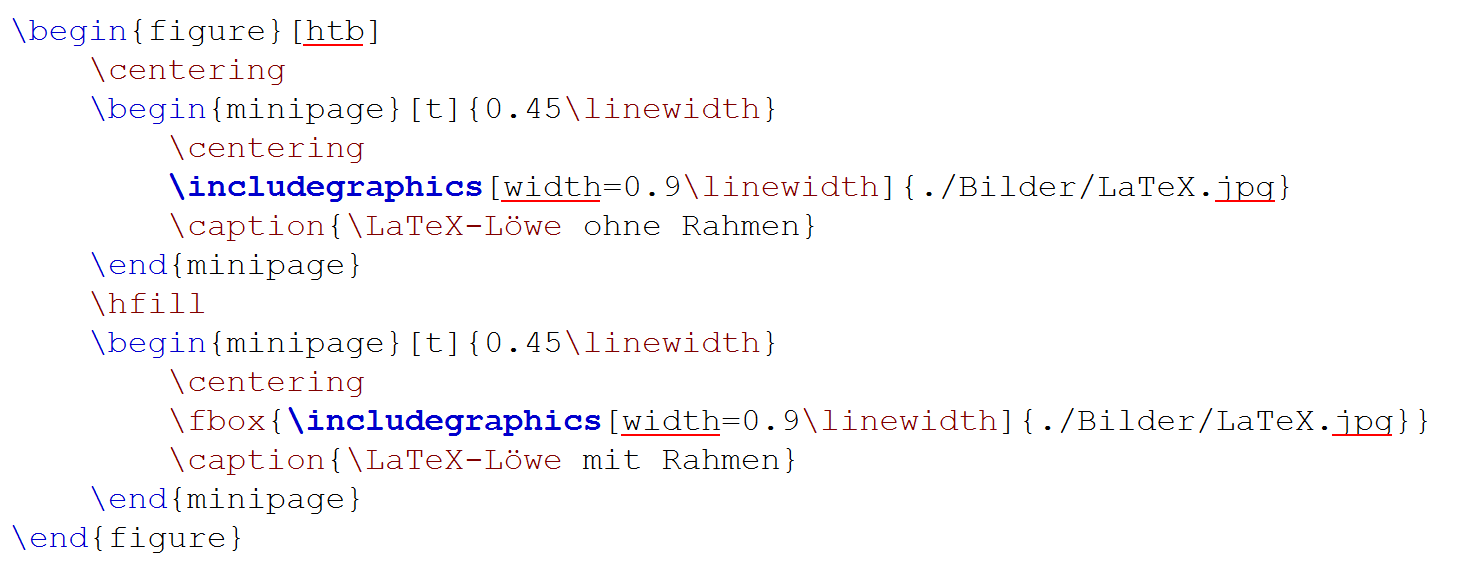
\includegraphics[width=0.9\textwidth]{./Bilder/BilderNebeneinander.png}}  
      \caption{Der \LaTeX-Code zu den beiden \LaTeX-Löwen}
\end{figure}

\vfill

Die vertikale Verteilung über die ganze Seite wird mit \code{\textbackslash{vfill}} erreicht. Der \LaTeX-Code für die Gestaltung der ganzen Seite (inkl. der konkreten Platzierung der \code{\textbackslash{vfill}}) ist in der Tex-Datei zu dieser Seite \code{./Inhalte/Inhalt\_Bilder.tex} zu sehen.


\end{spacing}
%
%
%
%
%
% ===== Kapitel 7 ======
%
\pagebreak 
\section{Arbeiten mit Abkürzungen}
\begin{spacing}{1.25}
In diesem Kapitel wird gezeigt, wie mit Abkürzungen gearbeitet wird.
\par
In einer wissenschaftlichen Arbeit dürfen oft wiederholte Begriffe durchaus abgekürzt werden. Die Verwendung von Abkürzungen sollte allerdings auf den Leserkreis abgestimmt sein. Neben den im Duden aufgeführten Abkürzungen dürfen auch Abkürzungen spezieller Fachtermini verwendet werden. Seien Sie sparsam mit Abkürzungen. Sie dürfen auf keinen Fall den Fluss Ihrer Arbeit stören.
\par
Wird auf die nachfolgend vorgestellte Art mit Abkürzungen gearbeitet, so kümmert sich LaTeX um die korrekte Verwendung von Abkürzungen (... einen Begriff bei erstmaliger Verwendung im Textabschnitt auszuschreiben und dabei die Abkürzung in Klammer zu setzen, bei allen weiteren Malen nur noch die Abkürzung einzusetzen ...). Natürlich lässt LaTeX verschiedene Arten der Übersteuerung dieses Verhaltens zu.
\par
Anders als Fachausdrücke, deren Bedeutung sich Fachfremden nicht auf den ersten Blick erschliesst, gehören allgemein übliche Ausdrücke wie 'z. B.' oder 'usw.' nicht in das Abkürzungsverzeichnis.
   
\end{spacing}
%
%
\subsection{Erfassen von Abkürzungen}
\begin{spacing}{1.25}
Alle Abkürzungen sind in einer separaten Datei mit Namen 'Abkuerzungen.tex' definiert. Diese Datei befindet sich im Verzeichnis 'Verzeichnisse' des Dokumentenordners.  Die Definitionen der Abkürzungen müssen mit folgendem Muster erstellt werden:
\begin{tcolorbox}[width=\textwidth,colback={light-gray},title={Erfassen von Abkürzungen},colbacktitle=gray,coltitle=white]
\begin{tabbing}
\code{\textbackslash{acro\{eth\}{[ETH]}\{Eidgenössische Technische Hochschule\}}}
\\
\small\code{\textbackslash{acro\{ethz\}{[ETHZ]}\{Eidgenössische Technische Hochschule Zürich\}}}
\\
\small\code{\textbackslash{acro\{epfl\}{[EPFL]}\{École polytechnique fédérale de Lausanne\}}}
\\
\small\code{\textbackslash{acro\{id\}{[ID]}\{Informatikdienste\}}}
\\
\small\code{\textbackslash{acro\{ppf\}{[PPF]}\{Procurement \& Portfolio Management\}}}
\\
\small\code{\indent\textbackslash{acro\{pm\}{[PM]}\{Portfolio Management\}}}
\end{tabbing}
\end{tcolorbox}

\end{spacing}
%
%
\subsection{Einsetzen von Abkürzungen}
\begin{spacing}{1.25}
Soll nun eine solche Abkürzung verwendet werden, geht das wie folgt.

\begin{tcolorbox}[width=\textwidth,colback={light-gray},title={Latex-Text},colbacktitle=gray,coltitle=white]

Ich bin angestellt an der \textcolor{red}{\textbackslash{ac\{eth\}}}, genauer an der \textcolor{red}{\textbackslash{ac\{ethz\}}}. Neben der \textcolor{red}{\textbackslash{ac\{ethz\}}} gibt es auch noch eine \textcolor{red}{\textbackslash{acs\{eth\}}} in der Westschweiz, nämlich die \textcolor{red}{\textbackslash{ac\{epfl\}}}. An der \textcolor{red}{\textbackslash{acs\{eth\}}} bin ich bei den \textcolor{red}{\textbackslash{ac\{id\}}} im Bereich \textcolor{red}{\textbackslash{ac\{pm\}}} tätig. Das \textcolor{red}{\textbackslash{ac\{pm\}}} ist eine Gruppe innerhalb der Sektion \textcolor{red}{\textbackslash{ac\{ppf\}}}.

\end{tcolorbox}


Die 'Norm' für die Verwendung von Abkürzungen sieht man mit der Verwendung der Abkürzung \textcolor{red}{\code{\textbackslash{ac\{ethz\}}}} an der zweiten und dritten Stelle im Text.


\begin{tcolorbox}[width=\textwidth,colback={light-gray},title={Print-Text},colbacktitle=gray,coltitle=white]

Ich bin angestellt an der \ac{eth}, genauer an der \ac{ethz}. Neben der \ac{ethz} gibt es auch noch eine \acs{eth} in der Westschweiz, nämlich die \ac{epfl}. An der \acs{eth} bin ich bei den \ac{id} im Bereich \ac{pm} tätig. Das \ac{pm} ist eine Gruppe innerhalb der Sektion \ac{ppf}.

\end{tcolorbox}

Am besten sieht man das, wenn im Latex Editor Texmaker die Tex-Datei geöffnet hat und man sich mit \keys{F1} die pdf Vorschau des Dokumentes anzeigen lässt.

\end{spacing}
%
%
\subsection{Verwenden von Abkürzungen}
\begin{spacing}{1.25}
Abkürzungen sollten in wissenschaftlichen Arbeiten, egal ob in Semester-, Prüfungs-, Bachelor- oder Masterarbeiten, möglichst spärlich und nur dann verwendet werden, wenn sie Klarheit und Lesbarkeit nicht beeinträchtigen. Dein angestrebter Leserkreis sollte sofort verstehen, was gemeint ist, oder es in einem vorangestellten Abkürzungsverzeichnis erklärt bekommen. 

Abkürzungen in Fachpublikationen sind i.d.R weniger Problematisch, sofern die verwendeten Abkürzungen im entsprechenden Fachbereich üblich sind.

Führe keine Abkürzung ein, die du nicht mindestens drei- oder viermal verwendest. Verwende stattdessen einfach den vollen Begriff.




\end{spacing}
%
%
%
%
%
% ===== Kapitel 8 ======
%
\pagebreak 
\section{Arbeiten mit Fussnoten}
\begin{spacing}{1.25}
Für die Verwendung von Fussnoten gelten folgende Regeln:


\begin{itemize} 
\item Fussnoten werden durch hochgestellte Ziffern nach dem Satzzeichen eines Absatzes bzw. Satzes oder nach einem zu zitierenden Wort angegeben. 

\item Mehrere Fussnoten an derselben Stelle sind nicht sinnvoll. 

\item Fussnoten gelten als ganze Sätze und müssen daher mit Grossbuchstaben begonnen und mit einem Punkt beendet werden. 

\item Gliederungsüberschriften dürfen nicht mit einer Fussnote versehen werden. 

\item Fussnoten gehören immer auf dieselbe Seite wie die Fussnotenreferenz im Text\footnote{Keine Regel ohne Ausnahme! In diesem Dokument werden alle Fussnoten am Ende des Dokumentes aufgeführt, um den Textfluss und das Seitenlayout nicht zu sehr zu stören.}. 

\item Ein Zitat aus einer anderen als der Originalquelle zu übernehmen (rezitieren) ist zu vermeiden.

\end{itemize}

Weiter sollte auch beachtet werden, dass die Arbeit auch ohne das Lesen der entsprechenden Fussnote verständlich sein muss. Daher gehören z.B. für die Argumentation wichtige Thesen nicht in eine Fussnote. Der in Fussnoten stehende Text sollte darum kurz und präzise sein. Exkurse sind zu vermeiden.

\end{spacing}
%
%
\subsection{Erfassen von Fussnoten}
\begin{spacing}{1.25}
Soll nun eine solche Fuss- (resp. Endnote) gesetzt werden, geht das wie folgt:

\begin{tcolorbox}[width=\textwidth,colback={light-gray},title={Latex-Text},colbacktitle=gray,coltitle=white]

An dieser Stelle \textcolor{red}{\textbackslash{footnote\{Fussnoten-Text\}}} wird eine Fussnote eingefügt.

\end{tcolorbox}


In diesem Dokument erscheint die Fussnote dann aber erst am Ende des Dokumentes, vor der eidesstattlichen Erklärung (siehe auch Inhaltsverzeichnis).

\begin{tcolorbox}[width=\textwidth,colback={light-gray},title={Print-Text},colbacktitle=gray,coltitle=white]

An dieser Stelle\footnote{Fussnoten-Text} wird eine Fussnote eingefügt.

\end{tcolorbox}

\end{spacing}
%
%
%
%
%
% ===== Kapitel 9 ======
%
\pagebreak 
\section{Arbeiten mit Stichworten}
\begin{spacing}{1.25}

Es ist im Rahmen einer wissenschaftlichen Arbeit i.d.R. nicht unbedingt erforderlich, ein Stichwortverzeichnis zu erstellen. Als erstes jedoch ein Beispiel mit etwas Text, der lediglich dazu dient einige Einträge im Stichwortverzeichnis zu erzeugen.

Auf dieser Seite sind die Begriffe System\index{System}, Systemzustand\index{System!Zustand}, Systemelement\index{System!Element} und Emergenz\index{Emergenz} von Interesse. Auf dieser Seite sei nochmals was gesagt zu System\index{System} und Systemelement\index{System!Element} sowie zu Transformationsprozess.\index{Transformationsprozess}

\textbf{Wichtige Hinweise:}  
\begin{itemize}[rightmargin=1.0cm]
\item{Das Stichwortverzeichnis muss separat erstellt werden. In Texmaker erfolgt dies mit der Funktionstaste \keys{F12}.} 
\item{Das Standard-Stichwortverzeichnis ist meines Erachtens nicht schön. Darum habe ich für dieses eine eigene Stil-Datei \code{index.ist} erstellt. Diese muss in der Konfiguration von Texmaker angegeben werden (siehe auch \cref{fig:Konfig}: \nameref{fig:Konfig} auf Seite \pageref{fig:Konfig}).}
\end{itemize}

\end{spacing}
%
%
\subsection{Erfassen von Stichworten}
\begin{spacing}{1.25}
Um einen Begriff (oder Namen) in das Stichwortverzeichnis aufzunehmen, wird der entsprechende Begriff (oder Namen)  wie folgt markiert:

\begin{tcolorbox}[width=\textwidth,colback={light-gray},title={Latex-Text},colbacktitle=gray,coltitle=white]

Die Begriffe System\textcolor{red}{\textbackslash{index\{System\}}}, Systemzustand\textcolor{red}{\textbackslash{index\{System!Zustand\}}} und Systemelement\textcolor{red}{\textbackslash{index\{System!Element\}}} sollen im Stichwortverzeichnis aufgenommen werden.

\end{tcolorbox}

Im gedruckten Text sieht das dann wie folgt aus:

\begin{tcolorbox}[width=\textwidth,colback={light-gray},title={Print-Text},colbacktitle=gray,coltitle=white]

Die Begriffe System\index{System}, Systemzustand\index{System!Zustand} und Systemelement\index{System!Element} sollen im Stichwortverzeichnis aufgenommen werden.

\end{tcolorbox}

Im gedruckten Text ist nicht zu erkennen, ob ein bestimmter Begriff (oder Name) im Stichwortverzeichnis aufgenommen wird.

\end{spacing}
%
%
%
%
%
% ===== Kapitel 10 ======
%
\pagebreak 
\section{Arbeiten mit Quellenangaben}
\begin{spacing}{1.25}

Quellenangaben und Zitate erfüllen in wissenschaftlichen Texten bzw. in wissenschaftlichen Arbeiten zwei Hauptziele\cite{NW2017}:

\begin{itemize}

\item[a)] Nachvollziehbarkeit der Argumentation, des (gedanklichen) Experiments
Ein wissenschaftlicher Beitrag kann nur dann weiterverwendet werden, wenn sich die Argumentation, das (gedankliche) Experiment für die Lesenden überprüfen lässt.

\item[b)] Unterscheidung zwischen eigenen und fremden Gedanken (geistiges Eigentum)
Ideen, Beispiele, ein bestimmtes methodisches Vorgehen, Bilder, Grafiken, Tabellen u.a., die aus anderen Texten stammen, müssen als fremdes geistiges Eigentum ausgewiesen werden.

\end{itemize}

\textbf{Wichtige Regel:} Quellenangaben gehören zum Satz dazu und stehen daher VOR dem Punkt bzw. Satzzeichen.

\end{spacing}
%
%
\subsection{Erfassen von Quellen}
\begin{spacing}{1.25}
Sämtliche (Literatur-) Quellen die im Dokument referenziert werden müssen in einer separaten Datei mit Endung \menu{*.bib} in einem speziellen Format erfasst werden.

\begin{figure}[h!]
\centering
  % 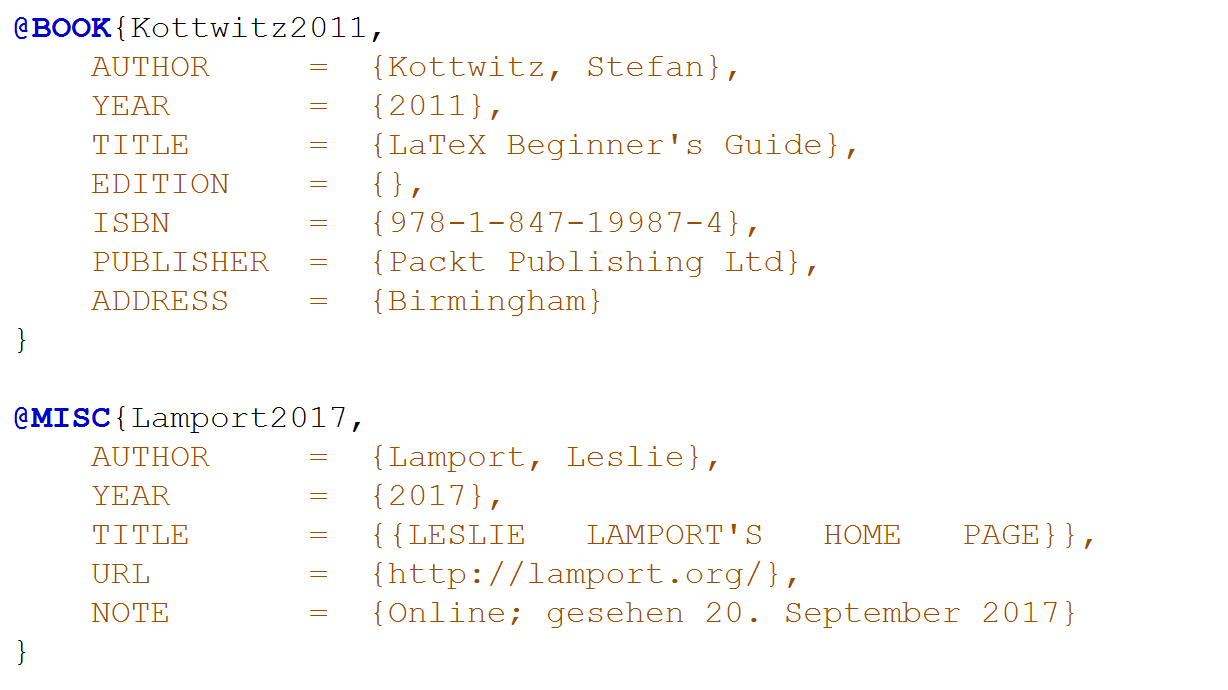
\includegraphics[width=0.75\textwidth]{./Bilder/QuellenErfassen.png}        % Bild ohne Rahmen
  \fbox{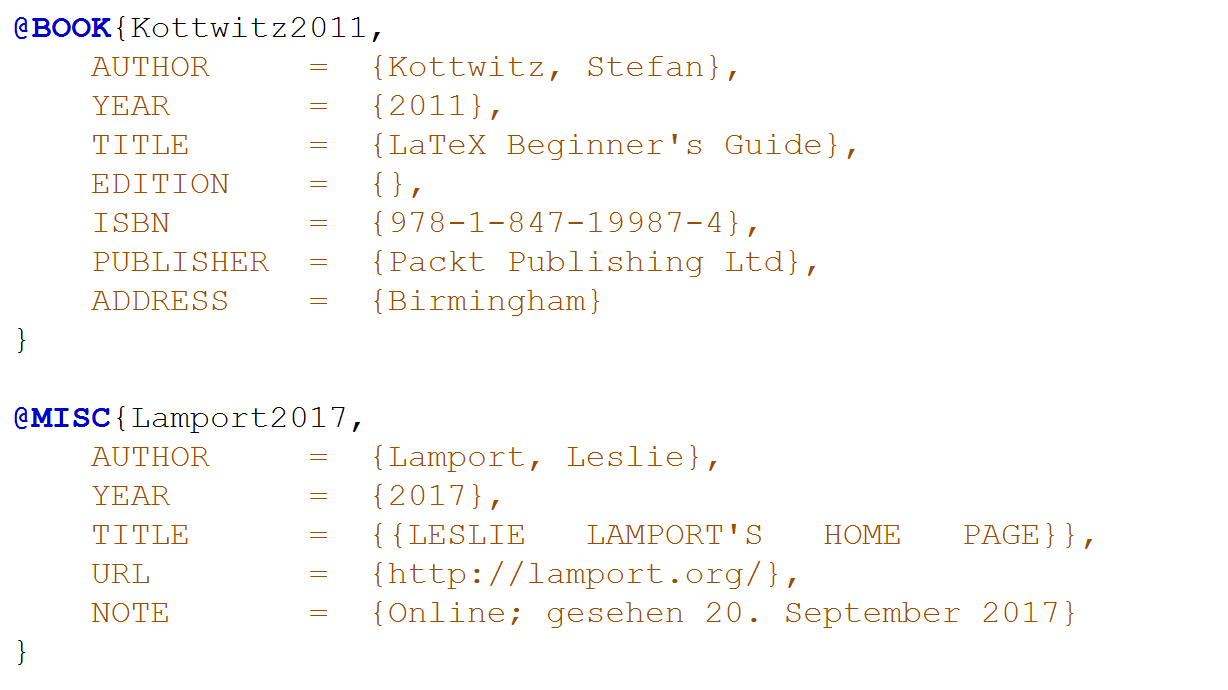
\includegraphics[width=0.75\textwidth]{./Bilder/QuellenErfassen.png}}   % Bild mit Rahmen
  \caption{Erfassen der Quellen}
  \label{fig:QuellenErfassen}
\end{figure} 

Auf der Internet-Seite \menu{\url{http://literatur-generator.de/}} kann man sich solche Einträge generieren lassen.

\end{spacing}
%
%
\subsection{Verwenden von Quellen}
\begin{spacing}{1.25}

Um auf eine verwende Quelle zu verweisen, wird der Verweis wie folgt eingesetzt:

\begin{tcolorbox}[width=\textwidth,colback={light-gray},title={Latex-Text},colbacktitle=gray,coltitle=white]

Are you ready to leave those ''what you see is what you get'' word processors behind and to enter the world of real, reliable, and high-quality typesetting\textcolor{red}{\textbackslash{cite\{Kottwitz2011\}}}?

\end{tcolorbox}

Im gedruckten Text sieht das dann wie folgt aus:

\begin{tcolorbox}[width=\textwidth,colback={light-gray},title={Print-Text},colbacktitle=gray,coltitle=white]

Are you ready to leave those ''what you see is what you get'' word processors behind and to enter the world of real, reliable, and high-quality typesetting\cite{Kottwitz2011}?

\end{tcolorbox}

\end{spacing}
%
%
\subsection{Quellenverzeichnis erstellen}
\begin{spacing}{1.25}

Die in der \menu{*.bib} Datei erfassten Informationen zu der Quelle sind im Literatur- / Quellenverzeichnis aufgeführt.

\begin{figure}[h!]
\centering
  % 
\includegraphics[width=0.75\textwidth]{./Bilder/QuellenVerzeichnis.png}        % Bild ohne Rahmen
  \fbox{
\includegraphics[width=0.75\textwidth]{./Bilder/QuellenVerzeichnis.png}}   % Bild mit Rahmen
  \caption{Auflistung der Quellen im Literatur- / Quellenverzeichnis}
  \label{fig:QuellenVerzeichnis}
\end{figure} 

Erstellt wird das Literatur- / Quellenverzeichnis mit folgendem Befehl:

\begin{figure}[h!]
\centering
  % 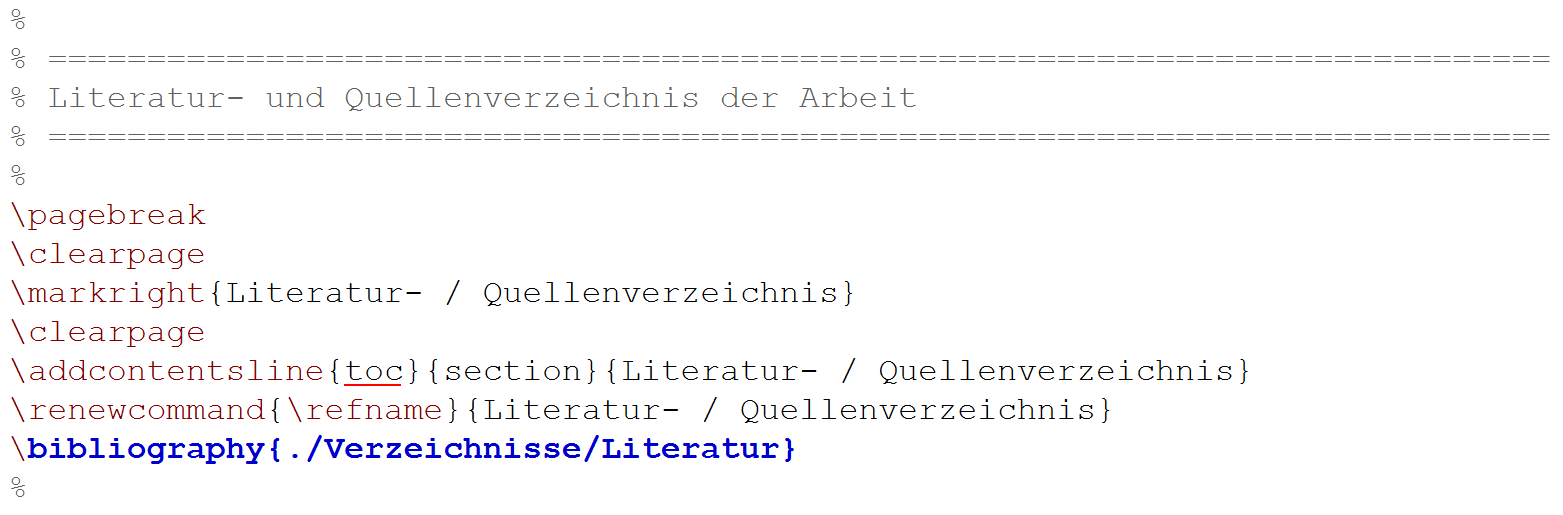
\includegraphics[width=0.75\textwidth]{./Bilder/QuellenVerzeichnisErstellen.png}        % Bild ohne Rahmen
  \fbox{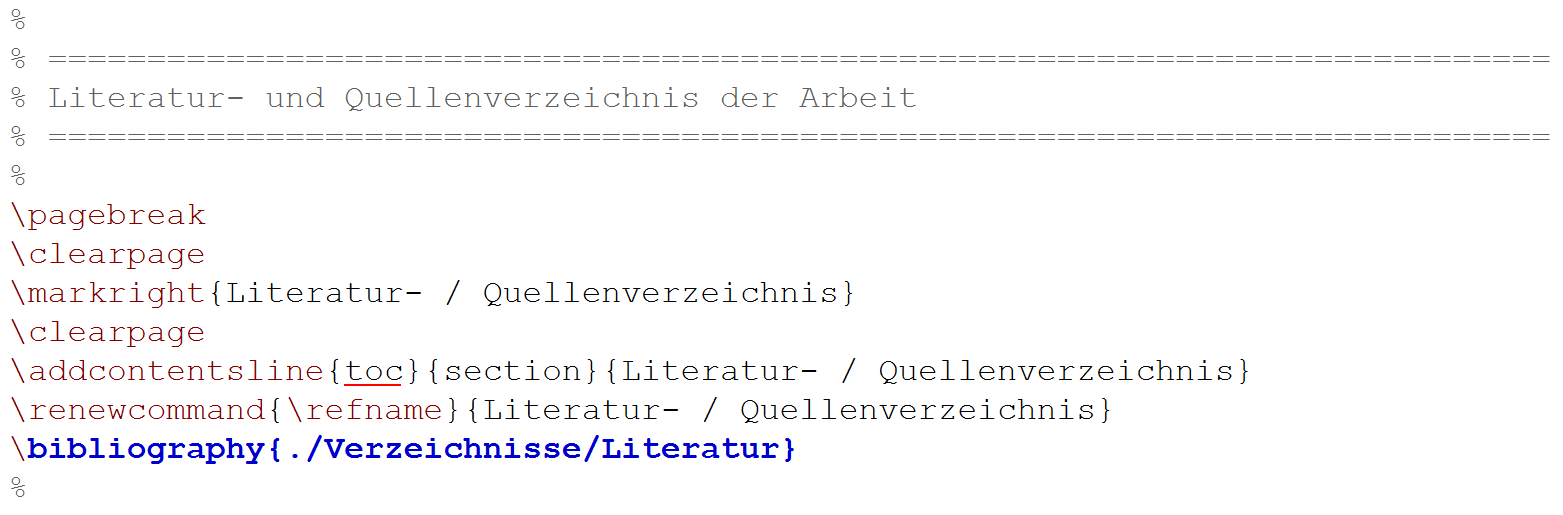
\includegraphics[width=0.75\textwidth]{./Bilder/QuellenVerzeichnisErstellen.png}}   % Bild mit Rahmen
  \caption{Erstellen des Literatur- / Quellenverzeichnis}
  \label{fig:QuellenVerzeichnisErstellen}
\end{figure} 

\end{spacing}
%
%
%
%
%
%
%
% ============================================================================
% ============================================================================
% ============================================================================
% Hier endet der eigentliche Inhalt des Dokumentes
%
% Nachfolgend kommen weitere formale Kapitel, die jedoch wieder ohne
% Kapitelnummer und mit römischer Seitenzahl geführt werden.
% ============================================================================
% ============================================================================
% ============================================================================
%
%
%
\pagebreak 
\clearpage
\pagenumbering{roman}
\setcounter{page}{\theSeitenzahlSpeicherRoman}
\addtocounter{page}{1}
\ofoot{\thepage{}}
%
%
%
% ============================================================================
% Ergänzende Materialien resp. Anhang der Arbeit
% ============================================================================
%
%
\markright{Ergänzende Materialien / Anhang}
\clearpage
\section*{Ergänzende Materialien / Anhang} 
\addcontentsline{toc}{section}{Ergänzende Materialien / Anhang}
\begin{spacing}{1.25}
An dieser Stelle können ergänzende Materialien und/oder Anhänge eingefügt werden.
\end{spacing}
%
%
%
% ============================================================================
% Literatur- und Quellenverzeichnis der Arbeit
% ============================================================================
%
\pagebreak 
\clearpage
\markright{Literatur- / Quellenverzeichnis}
\clearpage
\addcontentsline{toc}{section}{Literatur- / Quellenverzeichnis}
\renewcommand{\refname}{Literatur- / Quellenverzeichnis} 
% Für Biber
\printbibliography
% Für BibLaTex
%\bibliography{./Verzeichnisse/Literatur}
%
%
%
% ============================================================================
% Stichwort- und Namensverzeichnis der Arbeit
% ============================================================================
%
\pagebreak 
\clearpage
\markright{Stichwort- / Namensverzeichnis}
\clearpage
\addcontentsline{toc}{section}{Stichwort- / Namensverzeichnis}
\renewcommand{\indexname}{Stichwort- / Namensverzeichnis}
\printindex
%
%
%
% ============================================================================
% Die Fussnoten der Arbeit
% ============================================================================
%
\pagebreak 
\clearpage
\markright{Fussnoten}
\clearpage
\addcontentsline{toc}{section}{Fussnoten}
\renewcommand*{\notesname}{Fussnoten}
\begingroup 
\parindent 0pt 
\parskip 2ex 
\def\enotesize{\normalsize} 
\theendnotes 
\endgroup 
%
%
%
% ============================================================================
% Eidesstattliche Erklärung der Arbeit
% ============================================================================
%
\pagebreak 
\clearpage
\markright{Eidesstattliche Erklärung}
\clearpage
\section*{Eidesstattliche Erklärung} 
\addcontentsline{toc}{section}{Eidesstattliche Erklärung}
\begin{spacing}{1.25}
Hiermit erkläre ich, dass ich die vorliegende Arbeit mit Namen \textbf{\textit{\titel}} ohne Hilfe Dritter und ohne Benutzung anderer als der angegebenen Hilfsmittel angefertigt habe; die aus fremden Quellen direkt oder indirekt übernommenen Gedanken sind als solche kenntlich gemacht. Die Arbeit wurde bisher in gleicher oder ähnlicher Form in keiner anderen Prüfungsbehörde vorgelegt und auch noch nicht veröffentlicht.

\vspace{5cm}

\parbox{7cm}{\hrule
\strut \centering\footnotesize (Ort, Datum)} \hfill\parbox{7cm}{\hrule
\strut \centering\footnotesize (\autor, \mtrnr)}

\end{spacing}
%
%
%
\end{document}